\chapter{Experiments}
\label{sec:experiments}
In order to demonstrate the efficacy of the proposed method for estimating detection probability, numerous experiments were conducted. This section meticulously examines each of these experiments, delineating the selected parameters and conducting a comparative analysis against the GM-PHD filter with static detection probability.
A mixture of video was made to examine the experiments.
\begin{itemize}
  \item \textbf{V1:} This video shot by a camera from a highway was downloaded from YouTube. The link of this video: \href{https://www.youtube.com/watch?v=KBsqQez-O4w&t=30s&ab_channel=NickMartinez}{youtube.com}
  \item \textbf{V2:} The next video comes from YouTube as well. It captures a common traffic. The link of this video: \href{https://www.youtube.com/watch?v=7WFYiZersNc&ab_channel=AbdulMunaim}{youtube.com}
  \item \textbf{V3:} To get a video of a traffic with an obstacle in the view of the camera, we recorded a video on
  our own. This video is one of them.
 % \item \textbf{V4:} Another video, we recorded, with a slightly different scenario.
\end{itemize}

In all experiments as a state space model, CVM model is used, i.e., the state $x_k = [p_{x,k},p_{y,k},v_{x,k},v_{y,k}]^T$ of each target consists of two-dimensional position $(p_{x,k},p_{y,k})$ and velocity $(v_{x,k},v_{y,k})$. The measurement is the center of the mask of the detected object, which is typically noisy. The survival probability of the targets $p_{S,k} = 0.99$. A state evolution model \eqref{eq:phd_linear_model_state} is employed with
\begin{align}
  F_k &=
  \begin{bmatrix}
    I_2 & \Delta I_2 \\
    0_2 & I_2
  \end{bmatrix},
  \quad
  Q_k = \sigma_{\upsilon}^2
  \begin{bmatrix}
    \Delta I_4
  \end{bmatrix},
\end{align}
where $I_n$ and $0_n$ denote the $n\times n$ identity and zero matrices respectively and $\Delta = 1$ is the sampling
period.

For every experiment, different parameters for the model have to be applied. Parameters like $P, \sigma_{\upsilon}$
are displayed in corresponding tables.

The measurement follows the observation model \eqref{eq:phd_linear_model_measurements} with $H_k = [I_2, 0_2]$, $R_k
= \sigma_{\epsilon}^2I_2$, where $ \sigma_{\epsilon}$ is the standard deviation of the measurement noise.  $I_2$ and $0_2$ stand for
the $2\times 2$ identity and zero matrices, respectively.
The standard deviation $\sigma_{\epsilon}$ is displayed in tables as well.

Since the experiments compare the proposed method for estimating the dynamic detection probability with constant
detection probability, each table contains additional information about the necessary parameters. For constant
detection probability, it is the value of the probability. For dynamic detection probability, values of $T_H, T_C$
from Equation \eqref{eq:mphd_recursion_update_intesity_misdetect_pd}
and initial $p_{D,k}(x)$ is provided.

The pruning thresholds are the same for both GM-PHD filters, except filter with dynamic detection probability
includes second pruning threshold for pruning targets with state \textit{detected} or \textit{hidden}. The basic
pruning threshold is covered in tables as $T_p$, the lowered pruning threshold as $T_l$.

In addition, object detectors' results are dependent on thresholds as well. The Yolo model requires confidence threshold $T_{YOLO}$ for objects visualization. The Grounding DINO model requires two thresholds as it detects objects based on text input. The text input threshold $T_{text}$ and bounding box threshold $T_{bbox}$ for given experiment are included in corresponding parameter settings tables.

The labels above
the targets are the numerical representations of the state targets: $0=\text{detected}, 1=\text{hidden}, 2=\text{dead}$.

The means of the birth places are roughly in the middle of the traffic lanes and its confidence ellipses of size of
three standard
deviations are bounded by blue circles. The red bounding boxes in figures represent bounding
boxes
given by an object detection model. The red ellipses are the covariance matrices of the targets.


\section{E1: Traffic without any obstacle}
The first experiment focuses on comparison of GM-PHD filter with constant detection probability and GM-PHD filter
with dynamic detection probability with different settings explained in Section \ref{sec:mphd_problemDef}. To analyze,
if our proposed method works on common scenarios, videos do not include any obstacle, thus the targets are
constantly visible.



\section{E1: Traffic without any obstacle}
The first experiment focuses on the comparison of the GM-PHD filter with the constant detection probability and the GM-PHD
filter
with the dynamic detection probability with different settings explained in Section \ref{sec:mphd_problemDef}. To
analyze
if our proposed method works in common scenarios, videos do not include any obstacle, thus the targets are
constantly visible.

\subsection{V1}
The video \textit{V1} is recorded at 29 fps. For simplicity, only the detections of the right side of the traffic lanes are
taken into the account. Figures in Experiments E1-V1 -- E1-V3 show frames 36-79 of the video \textit{V1}, as they
include some interesting situations.
\subsection{V1 -- GM-PHD with the constant detection probability}
The measurements for the GM-PHD filter with the constant detection probability are obtained by the YOLO object detection
model. The parameters' values are displayed in Table \ref{tab:E1-V1-S0}.
\begin{table}[!h]
    \centering
    \begin{tabular}{|c|c|c|c|c|c|}
        \hline
        $P_{D}$ & $P$ & $\sigma_{\upsilon}$ & $\sigma_{\epsilon}$ & $T_p$ & $T_{YOLO}$ \\ \noalign{\hrule height 1.5pt}
        0.9 & $\diag(600,600,600,600)$ & 0.1 & 150 & 0.1 & 0.3\\
        \hline
    \end{tabular}
    \caption{The parameter settings for Experiment E1-V1 with the constant detection probability.}
    \label{tab:E1-V1-S0}
\end{table}

Figure \ref{fig:E1-V1-S0} shows some highlights of the GM-PHD filter with the constant detection probability.
\begin{itemize}
    \item \textbf{\ref{fig:E1-V1-S0:01}:} This frame marks the initial state, where four cars have been previously
    identified, thus representing our observed targets. In the distance, YOLO detects another car which, however,
    has not yet crossed any spawning point, so it is not included in the observed targets set.
    \item \textbf{\ref{fig:E1-V1-S0:02}:} A new car approaches the scene and is expected to be initialized soon. The
    YOLO model, although overall reliable, occasionally misses certain objects, as demonstrated here with the
    car on the left. With a detection probability of 0.9, this target is pruned from the set and considered lost.
    \item \textbf{\ref{fig:E1-V1-S0:03}:} The previously lost car is, once again, detected. However, it no longer
    falls within the set of observed targets.
    \item \textbf{\ref{fig:E1-V1-S0:04}:} Even though the newly arrived car has crossed the spawning point, the YOLO model
    consistently
    fails to detect it over several frames, resulting in its complete absence from tracking.
    \item \textbf{\ref{fig:E1-V1-S0:05}:} The two cars on the right evade the detection. On this occasion, one
    of the targets manages to persist, allowing for continued tracking of at least one car.
    \item \textbf{\ref{fig:E1-V1-S0:06}:} The previously undetected cars reappear in the frame. Both cars are
    successfully tracked once again.
    \item \textbf{\ref{fig:E1-V1-S0:07}:} Another car enters the scene and is promptly detected and initialized.
    \item \textbf{\ref{fig:E1-V1-S0:08}:} Despite YOLO detecting all the six cars, only three targets are visible in the
    scene. One of the targets encompasses two cars simultaneously, indicating that the GM-PHD filter effectively covers four out of the six targets.
\end{itemize}

In Figure \ref{gr:E1-V1-S0} it is clearly seen that even though the number of targets is increasing, the misdetection
of the YOLO model causes the targets' loss. The "All targets in set" line is fully covered by the blue line, thus the
targets are permanently lost and can not be reborn by a measurement.

This experiment shows that the GM-PHD filter is able to accurately track the position of objects. With the detection
probability $p_D = 0.9$ and without the modified pruning technique, the filter is very sensitive to the capability of
the
object detector and if YOLO is not able to detect all the desired objects, targets can be easily lost.

\begin{figure}[H]
    \centering
    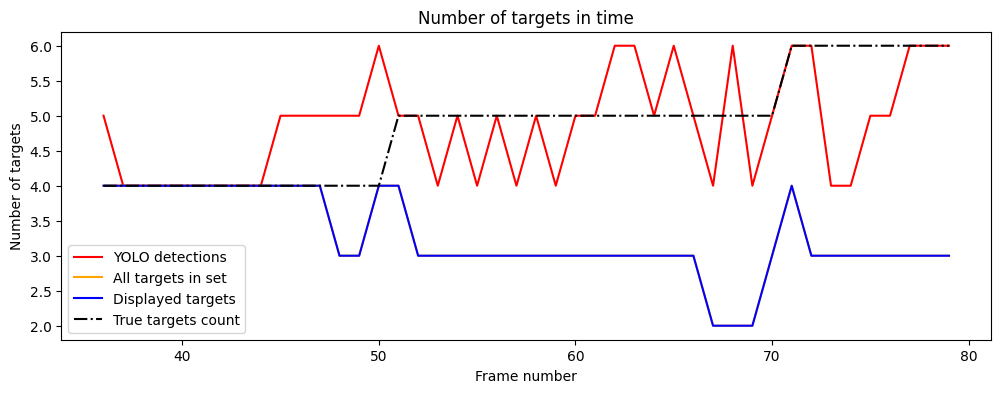
\includegraphics[width=\linewidth]{../../../experiments/E1/V1/noPd/staticPd_det}
    \caption{Development chart of number of detected targets, targets in the filter's queue, displayed targets and
    the true
    targets' count.}
    \label{gr:E1-V1-S0}
\end{figure}

\begin{figure}[H]
    \centering
    \begin{subfigure}{0.48\textwidth}
        \centering
        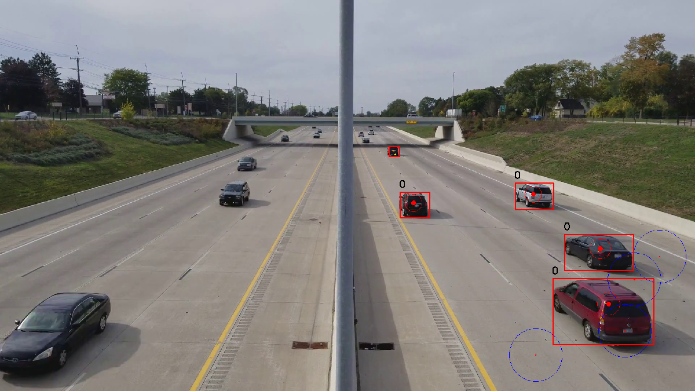
\includegraphics[width=\linewidth]{../../../experiments/E1/V1/noPd/36}
        \caption{Frame number: 36.}
        \label{fig:E1-V1-S0:01}
    \end{subfigure}
    \begin{subfigure}{0.48\textwidth}
        \centering
        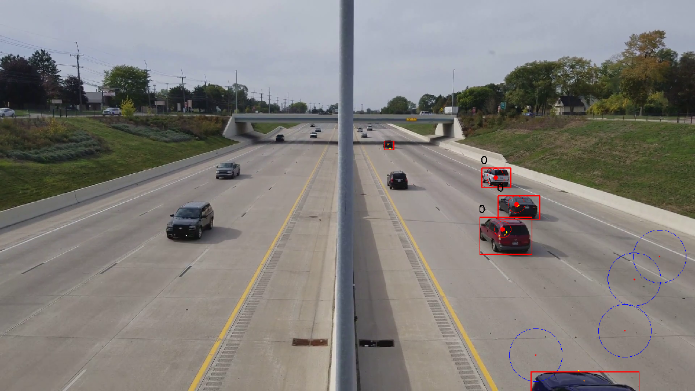
\includegraphics[width=\linewidth]{../../../experiments/E1/V1/noPd/48}
        \caption{Frame number: 48.}
        \label{fig:E1-V1-S0:02}
    \end{subfigure}
    \\
    \begin{subfigure}{0.48\textwidth}
        \centering
        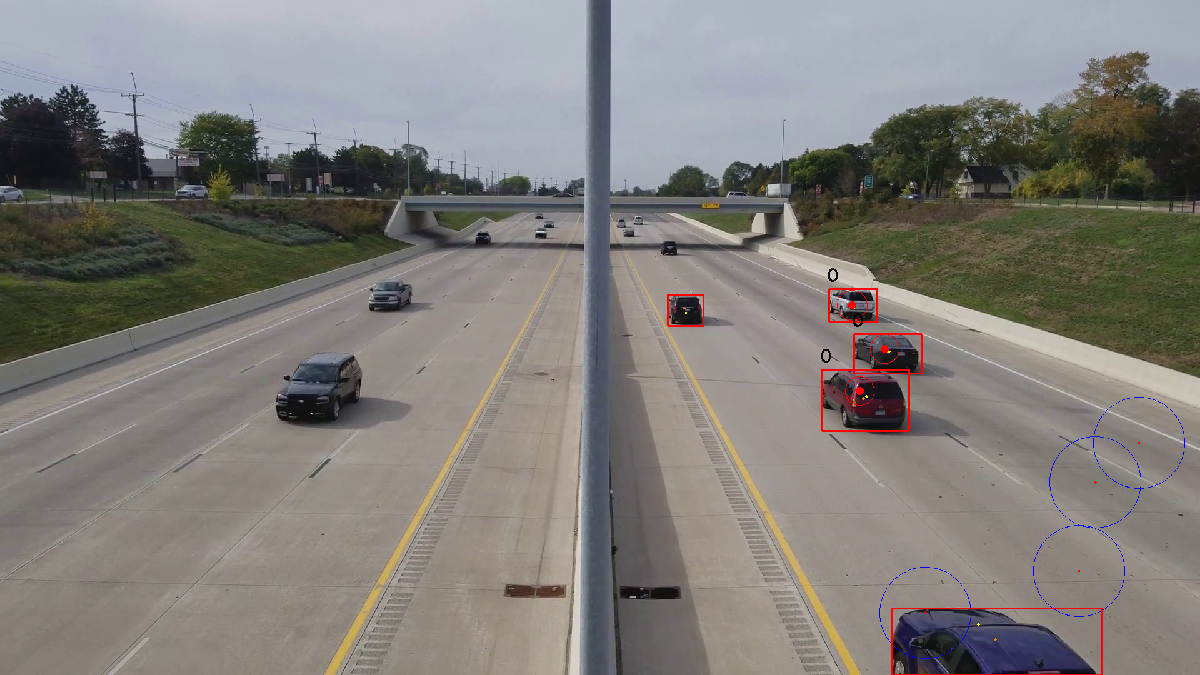
\includegraphics[width=\linewidth]{../../../experiments/E1/V1/noPd/49}
        \caption{Frame number: 49.}
        \label{fig:E1-V1-S0:03}
    \end{subfigure}
    \begin{subfigure}{0.48\textwidth}
        \centering
        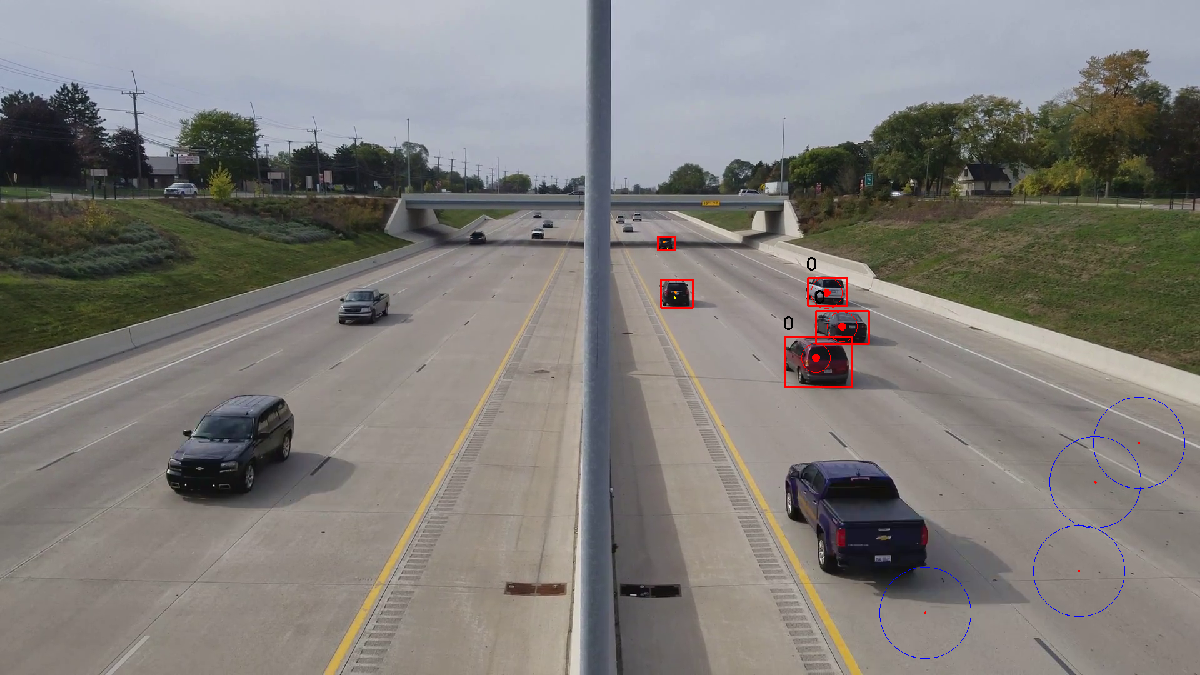
\includegraphics[width=\linewidth]{../../../experiments/E1/V1/noPd/56}
        \caption{Frame number: 56.}
        \label{fig:E1-V1-S0:04}
    \end{subfigure}
    \\
    \begin{subfigure}{0.48\textwidth}
        \centering
        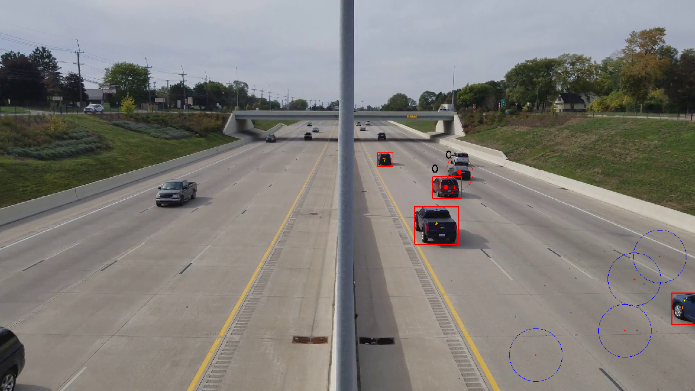
\includegraphics[width=\linewidth]{../../../experiments/E1/V1/noPd/67}
        \caption{Frame number: 67.}
        \label{fig:E1-V1-S0:05}
    \end{subfigure}
    \begin{subfigure}{0.48\textwidth}
        \centering
        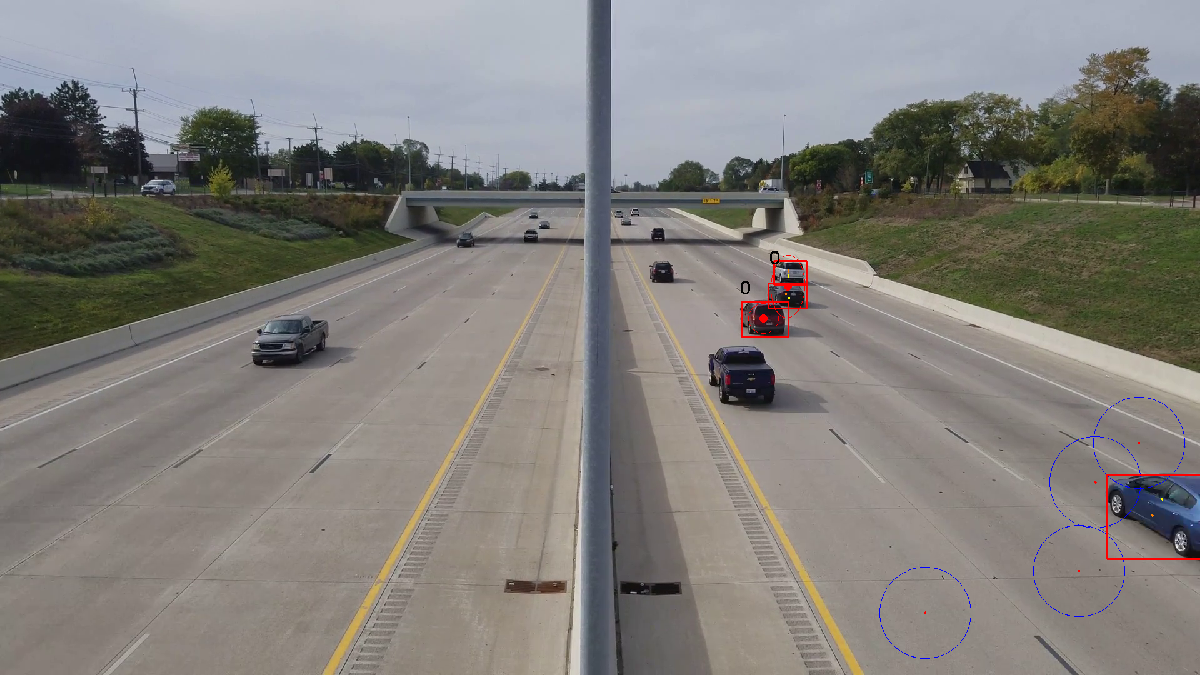
\includegraphics[width=\linewidth]{../../../experiments/E1/V1/noPd/69}
        \caption{Frame number: 69.}
        \label{fig:E1-V1-S0:06}
    \end{subfigure}
    \\
    \begin{subfigure}{0.48\textwidth}
        \centering
        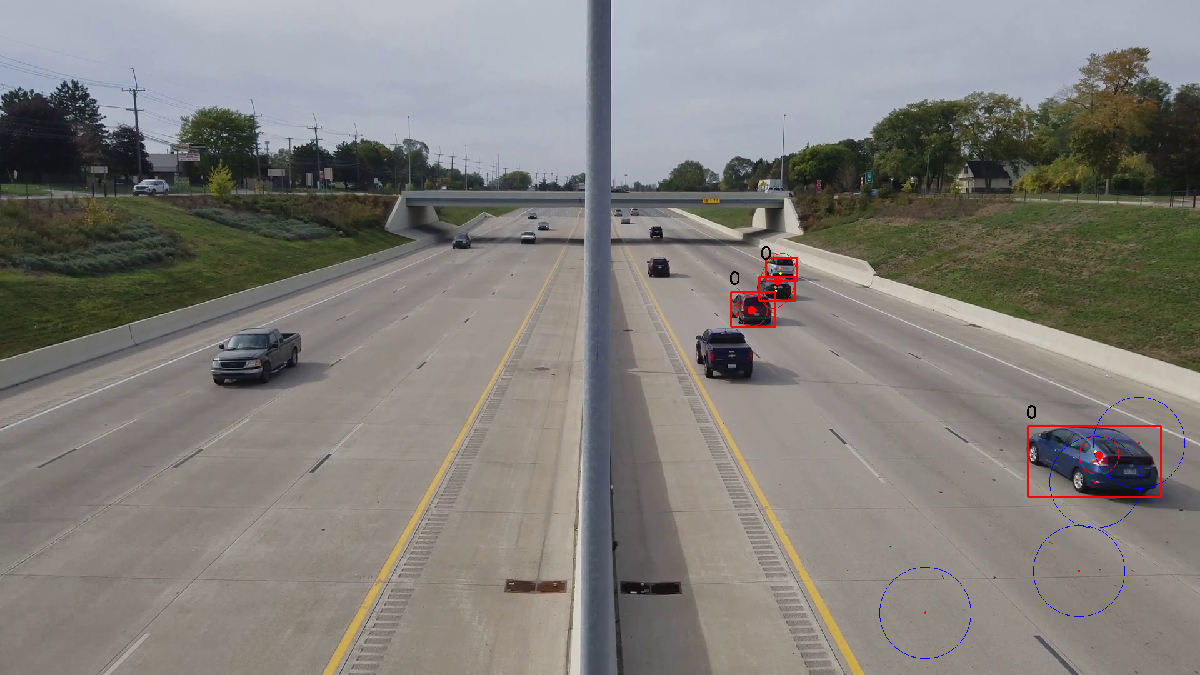
\includegraphics[width=\linewidth]{../../../experiments/E1/V1/noPd/73}
        \caption{Frame number: 73.}
        \label{fig:E1-V1-S0:07}
    \end{subfigure}
    \begin{subfigure}{0.48\textwidth}
        \centering
        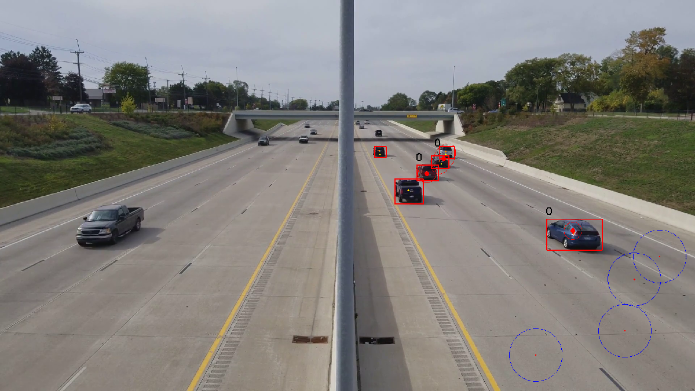
\includegraphics[width=\linewidth]{../../../experiments/E1/V1/noPd/79}
        \caption{Frame number: 79.}
        \label{fig:E1-V1-S0:08}
    \end{subfigure}
    \caption{Image sequence of tracked objects using the GM-PHD filter with the constant detection probability.}
    \label{fig:E1-V1-S0}
\end{figure}

\subsection{V1 -- GM-PHD with the dynamic detection probability}
The following experiments test the GM-PHD filter with the dynamic detection probability and the modified pruning in the
video \textit{V1}.
\subsubsection{S1 -- YOLO + YOLO}
This experiment enhances settings \textit{S1}, i.e, the YOLO model provides both object detection bboxes and
segmentation masks.
The parameter settings are shown in Table \ref{tab:E1-V1-S1}.
\begin{table}[H]
    \centering
    \begin{tabular}{|c|c|c|c|c|c|c|c|c|}
        \hline
        $P_{D,k}(x)$ & $P$ & $\sigma_{\upsilon}$ & $\sigma_{\epsilon}$ & $T_H$ & $T_d$ & $T_p$ & $T_l$ & $T_{YOLO}$ \\ \noalign{\hrule
        height 1.5pt}
        0.3 & $\diag(600,600,600,600)$ & 0.1 & 150 & 1 & 3 & 0.1 & 0.01 & 0.3\\
        \hline
    \end{tabular}
    \caption{The parameter settings for Experiment E1-V1-S1 with the dynamic detection probability.}
    \label{tab:E1-V1-S1}
\end{table}

Figure \ref{fig:E1-V1-S1} illustrates the performance of the GM-PHD filter under the dynamic detection probability and
settings \textit{S1}.

\begin{itemize}
    \item \textbf{\ref{fig:E1-V1-S1:01}:} Similarly as in the previous experiment, the initial frame presents four
    previously detected cars. Although a distant car is detected, it remains uninitialized since it has not crossed any spawning point.
    \item \textbf{\ref{fig:E1-V1-S1:02}:} By frame 48, the car on the left, which was undetected in the previous
    experiment, remains so. However, due to the elevated detection probability and adjusted pruning, the target manages to persist.
    \item \textbf{\ref{fig:E1-V1-S1:03}:} Despite the previous misdetections, the previously undetected car is once
    again
    identified, and the target successfully survives.
    \item \textbf{\ref{fig:E1-V1-S1:04}:} A new car crosses the spawning point, yet the YOLO model consistently fails to detect it over numerous consecutive frames, resulting in its non-initialization.
    \item \textbf{\ref{fig:E1-V1-S1:05}:} Two cars on the right evade the detection, yet their respective targets
    remain.
    \item \textbf{\ref{fig:E1-V1-S1:06}:} The previously undetected cars are once again identified, and both targets
    receive measurements, augmenting their weights.
    \item \textbf{\ref{fig:E1-V1-S1:07}:} Another car enters the scene and is successfully initialized.
    \item \textbf{\ref{fig:E1-V1-S1:08}:} The previously undetected car on the left merges with other targets.
    Consequently, this target is initialized despite the previous frequent misdetections. As a result, six true targets
    and six tracked targets are present.
\end{itemize}


The graph presented in Figure \ref{gr:E1-V1-S1} shows the enhanced performance of the GM-PHD filter. While all
targets do not immediately appear in the scene upon detection, they often still exist in the queue of targets
whose weights
have
not reached a threshold for display. However, upon receiving measurements, these targets' weights increase, leading to their reappearance in the scene.

This improvement is notable not only in the alignment of displayed targets with the true target count, but also in
the queue of potential targets exceeding the true count. Consequently, we gain awareness of potential targets that may manifest in the scene.


\begin{figure}[H]
    \centering
    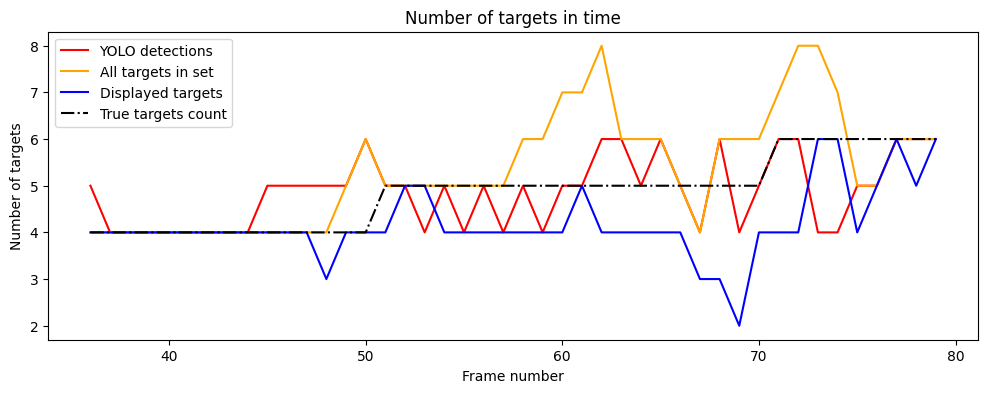
\includegraphics[width=\linewidth]{../../../experiments/E1/V1/YOLO/yolo_det}
    \caption{Development chart of the number of detected targets, targets in the filter's queue, displayed targets and
    the true
    targets' count.}
    \label{gr:E1-V1-S1}
\end{figure}

\begin{figure}[H]
    \centering
    \begin{subfigure}{0.48\textwidth}
        \centering
        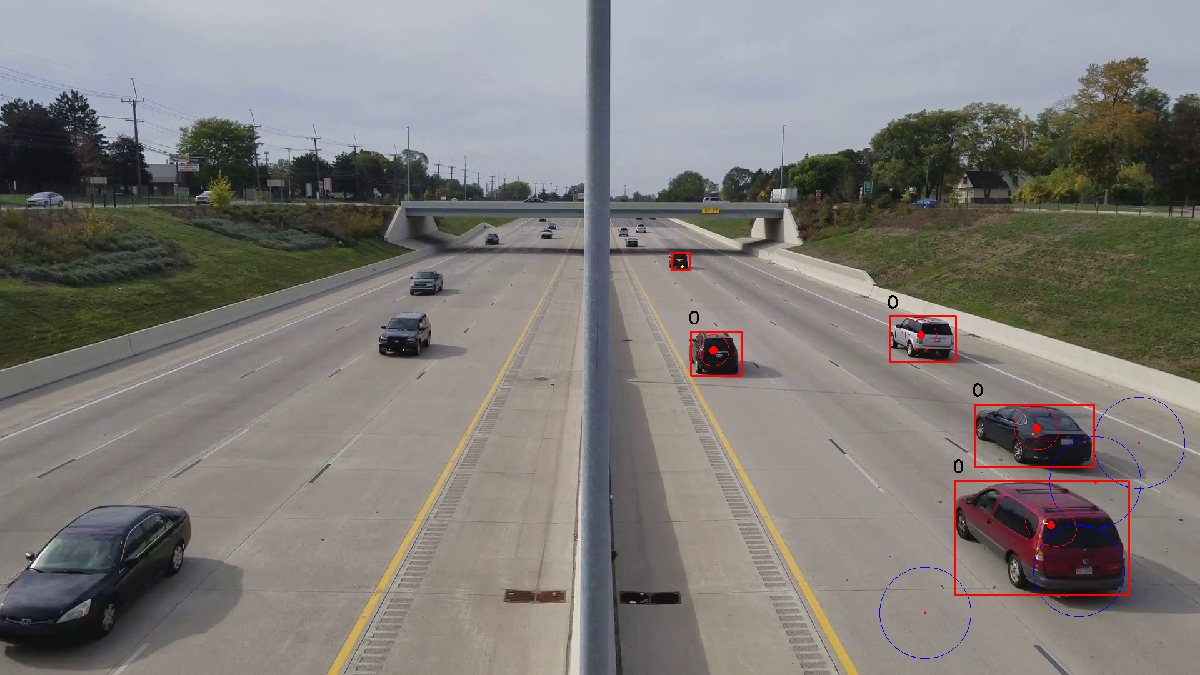
\includegraphics[width=\linewidth]{../../../experiments/E1/V1/YOLO/36}
        \caption{Frame number: 36.}
        \label{fig:E1-V1-S1:01}
    \end{subfigure}
    \begin{subfigure}{0.48\textwidth}
        \centering
        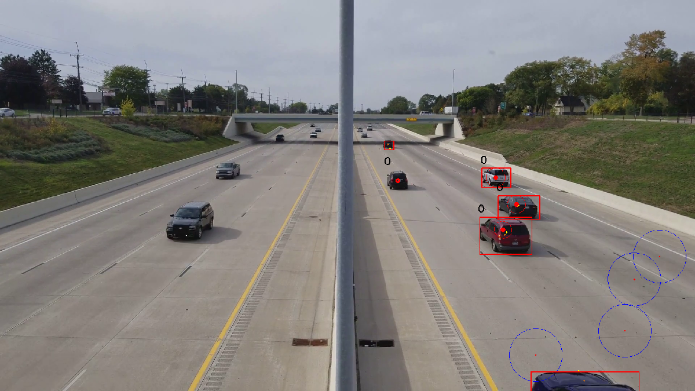
\includegraphics[width=\linewidth]{../../../experiments/E1/V1/YOLO/48}
        \caption{Frame number: 48.}
        \label{fig:E1-V1-S1:02}
    \end{subfigure}
    \\
    \begin{subfigure}{0.48\textwidth}
        \centering
        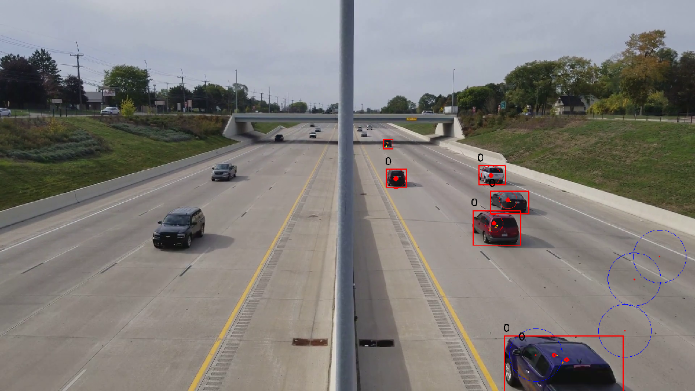
\includegraphics[width=\linewidth]{../../../experiments/E1/V1/YOLO/50}
        \caption{Frame number: 50.}
        \label{fig:E1-V1-S1:03}
    \end{subfigure}
    \begin{subfigure}{0.48\textwidth}
        \centering
        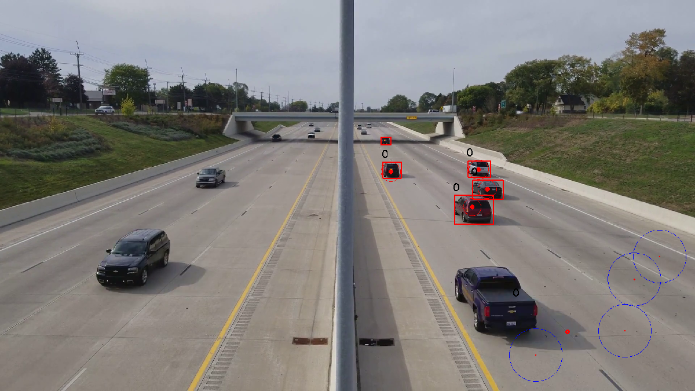
\includegraphics[width=\linewidth]{../../../experiments/E1/V1/YOLO/56}
        \caption{Frame number: 56.}
        \label{fig:E1-V1-S1:04}
    \end{subfigure}
    \\
    \begin{subfigure}{0.48\textwidth}
        \centering
        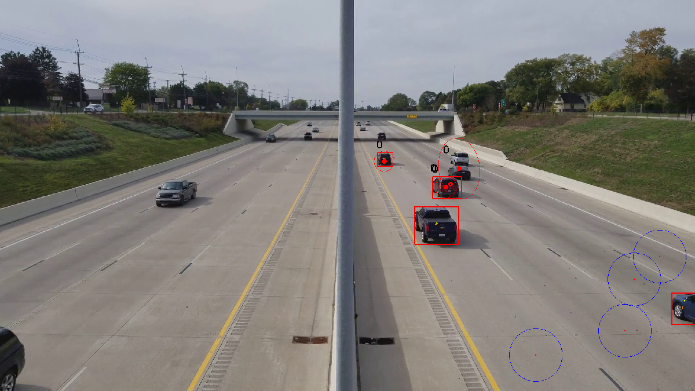
\includegraphics[width=\linewidth]{../../../experiments/E1/V1/YOLO/67}
        \caption{Frame number: 67.}
        \label{fig:E1-V1-S1:05}
    \end{subfigure}
    \begin{subfigure}{0.48\textwidth}
        \centering
        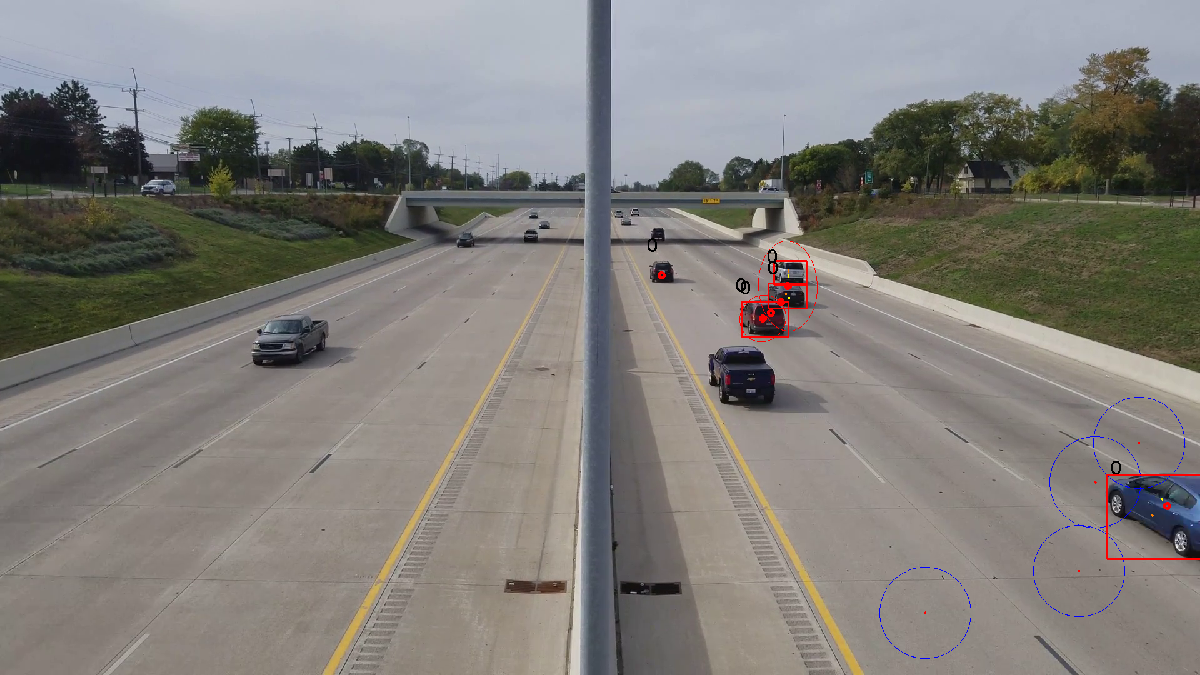
\includegraphics[width=\linewidth]{../../../experiments/E1/V1/YOLO/69}
        \caption{Frame number: 69.}
        \label{fig:E1-V1-S1:06}
    \end{subfigure}
    \\
    \begin{subfigure}{0.48\textwidth}
        \centering
        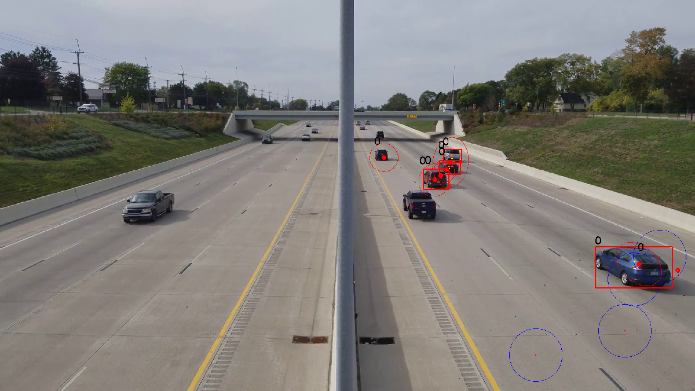
\includegraphics[width=\linewidth]{../../../experiments/E1/V1/YOLO/73}
        \caption{Frame number: 73.}
        \label{fig:E1-V1-S1:07}
    \end{subfigure}
    \begin{subfigure}{0.48\textwidth}
        \centering
        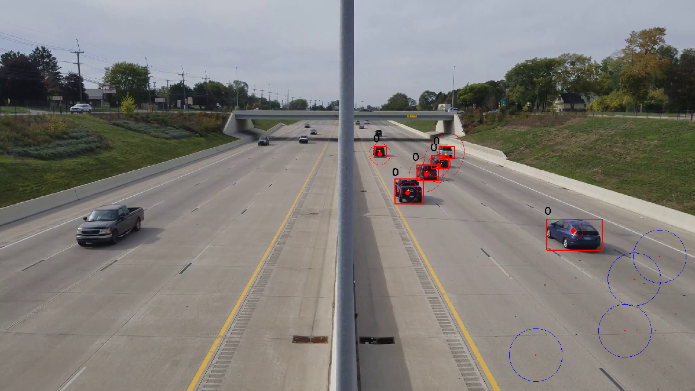
\includegraphics[width=\linewidth]{../../../experiments/E1/V1/YOLO/79}
        \caption{Frame number: 79.}
        \label{fig:E1-V1-S1:08}
    \end{subfigure}
    \caption{Image sequence of tracked objects using the GM-PHD filter with the dynamic detection probability and YOLO
    only.}
    \label{fig:E1-V1-S1}
\end{figure}







\subsubsection{S2 -- YOLO + SAM}
This experiment employs configuration \textit{S2}, wherein the YOLO model furnishes objects' bounding boxes and the SAM model furnishes segmentation masks.
The parameter configurations can be found in Table \ref{tab:E1-V1-S2}.
\begin{table}[H]
    \centering
    \begin{tabular}{|c|c|c|c|c|c|c|c|c|}
        \hline
        $P_{D,k}(x)$ & $P$ & $\sigma_{\upsilon}$ & $\sigma_{\epsilon}$ & $T_H$ & $T_d$ & $T_p$ & $T_l$ & $T_{YOLO}$ \\ \noalign{\hrule
        height 1.5pt}
        0.3 & $\diag(600,600,600,600)$ & 0.1 & 150 & 1 & 3 & 0.1 & 0.01 & 0.3\\
        \hline
    \end{tabular}
    \caption{The parameter settings for Experiment E1-V1-S2 with the dynamic detection probability.}
    \label{tab:E1-V1-S2}
\end{table}

Figure \ref{fig:E1-V1-S2} illustrates the GM-PHD filter's performance with the dynamic detection probability, employing
settings \textit{S2}.
This sequence is very similar to the previous experiment. There are four targets at the beginning and they are
tracked successfully the whole time. In the frame \ref{fig:E1-V1-S2:06} two of the targets are not detected, but both
survive. The YOLO model is not able to detect the fifth car, but it is initialized later due to the other target.

Figure \ref{gr:E1-V1-S2} shows a better stability in keeping the number of tracked targets. This might be caused by
the fact,
that the object detection YOLO model gives slightly different results than the object detection YOLO model with
segmentation capabilities. Furthermore, the "All targets in set" orange line, representing the number of targets in the
filter's queue, is more
accurate to the true count, deflecting only by one target at maximum.

Settings \textit{S2} perform manage a slightly better performance than settings \textit{S1}. The number of tracked
objects
is closer to
the true count.

\begin{figure}[H]
    \centering
    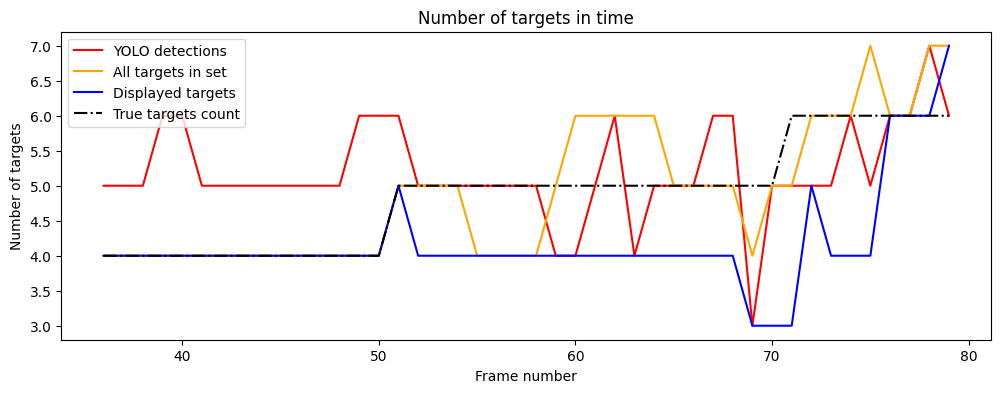
\includegraphics[width=\linewidth]{../../../experiments/E1/V1/SAM/sam_det}
    \caption{Development chart of the number of detected targets, targets in the filter's queue, displayed targets and
    the true
    targets' count.}
    \label{gr:E1-V1-S2}
\end{figure}

\begin{figure}[H]
    \centering
    \begin{subfigure}{0.48\textwidth}
        \centering
        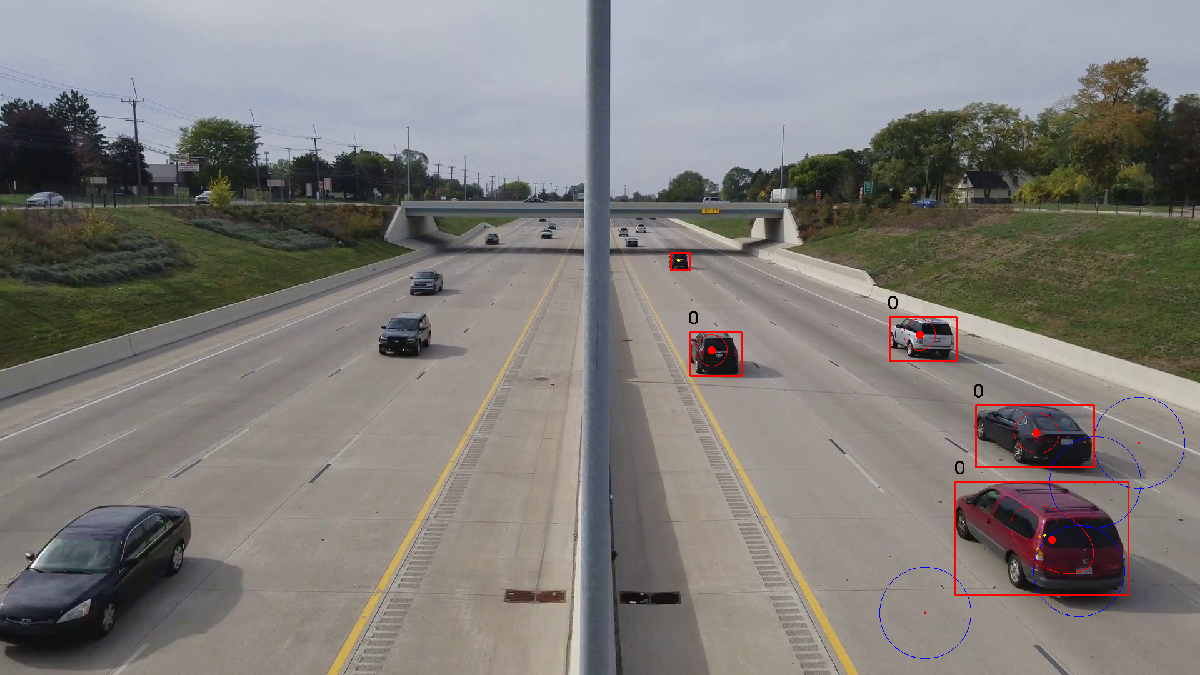
\includegraphics[width=\linewidth]{../../../experiments/E1/V1/SAM/36}
        \caption{Frame number: 36.}
        \label{fig:E1-V1-S2:01}
    \end{subfigure}
    \begin{subfigure}{0.48\textwidth}
        \centering
        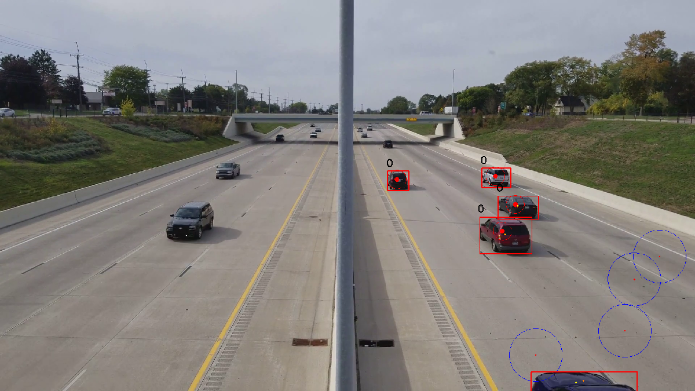
\includegraphics[width=\linewidth]{../../../experiments/E1/V1/SAM/48}
        \caption{Frame number: 48.}
        \label{fig:E1-V1-S2:02}
    \end{subfigure}
    \\
    \begin{subfigure}{0.48\textwidth}
        \centering
        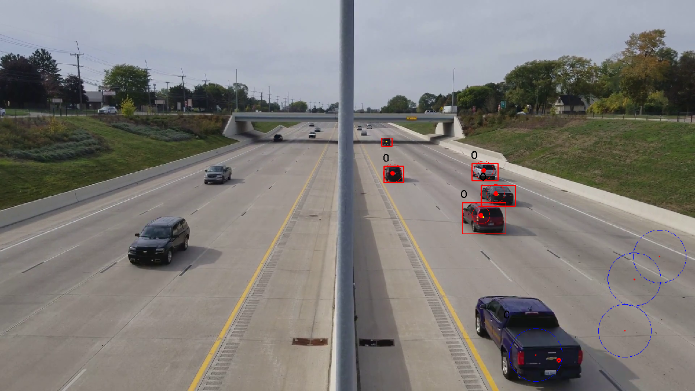
\includegraphics[width=\linewidth]{../../../experiments/E1/V1/SAM/53}
        \caption{Frame number: 53.}
        \label{fig:E1-V1-S2:03}
    \end{subfigure}
    \begin{subfigure}{0.48\textwidth}
        \centering
        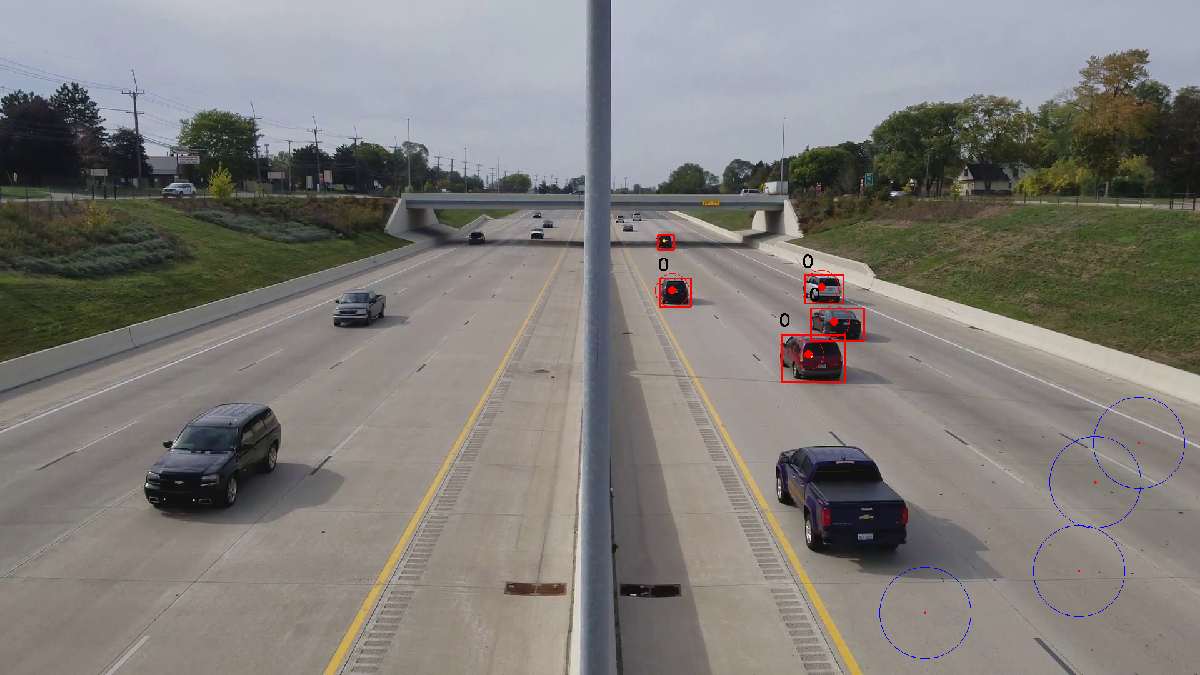
\includegraphics[width=\linewidth]{../../../experiments/E1/V1/SAM/57}
        \caption{Frame number: 57.}
        \label{fig:E1-V1-S2:04}
    \end{subfigure}
    \\
    \begin{subfigure}{0.48\textwidth}
        \centering
        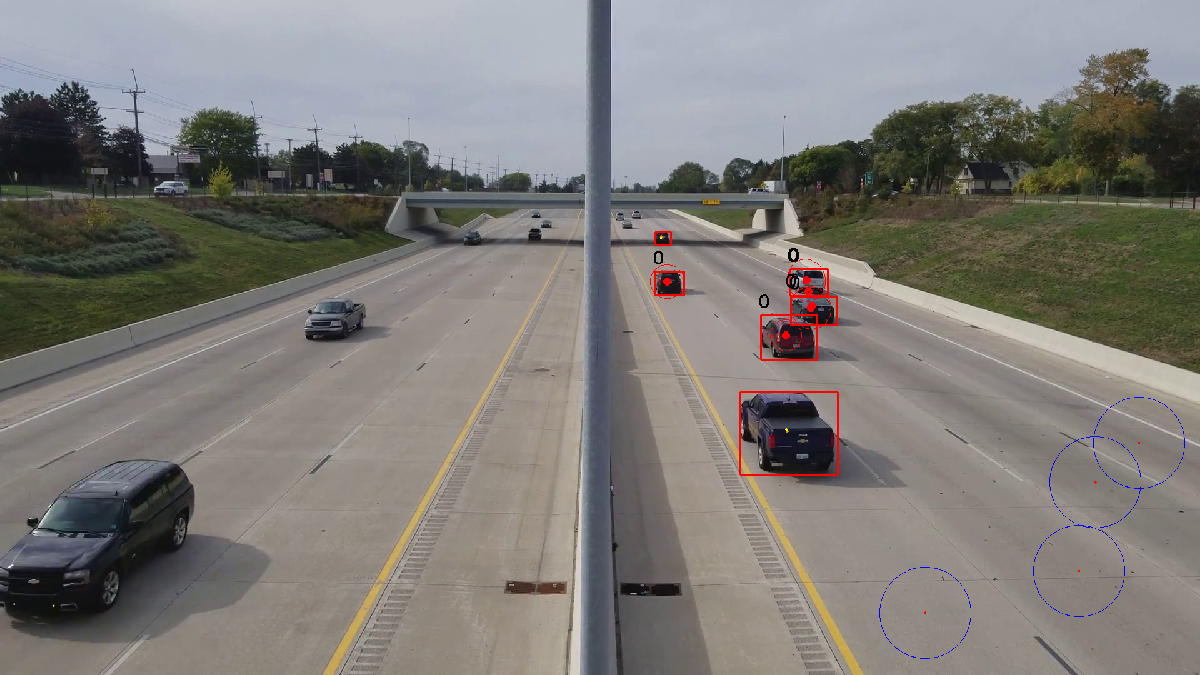
\includegraphics[width=\linewidth]{../../../experiments/E1/V1/SAM/62}
        \caption{Frame number: 62.}
        \label{fig:E1-V1-S2:05}
    \end{subfigure}
    \begin{subfigure}{0.48\textwidth}
        \centering
        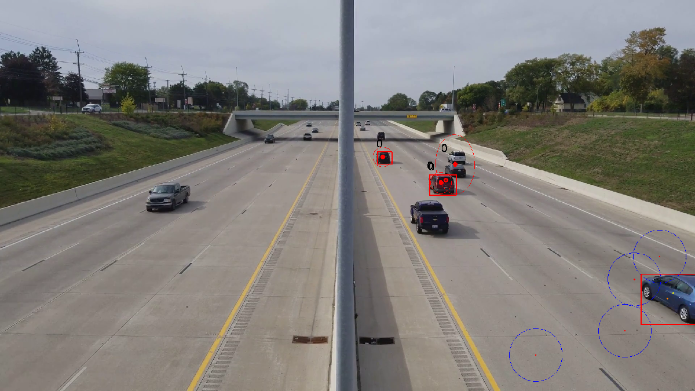
\includegraphics[width=\linewidth]{../../../experiments/E1/V1/SAM/69}
        \caption{Frame number: 69.}
        \label{fig:E1-V1-S2:06}
    \end{subfigure}
    \\
    \begin{subfigure}{0.48\textwidth}
        \centering
        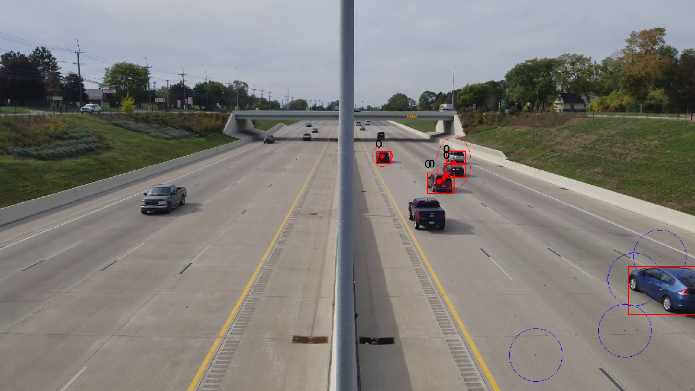
\includegraphics[width=\linewidth]{../../../experiments/E1/V1/SAM/70}
        \caption{Frame number: 70.}
        \label{fig:E1-V1-S2:07}
    \end{subfigure}
    \begin{subfigure}{0.48\textwidth}
        \centering
        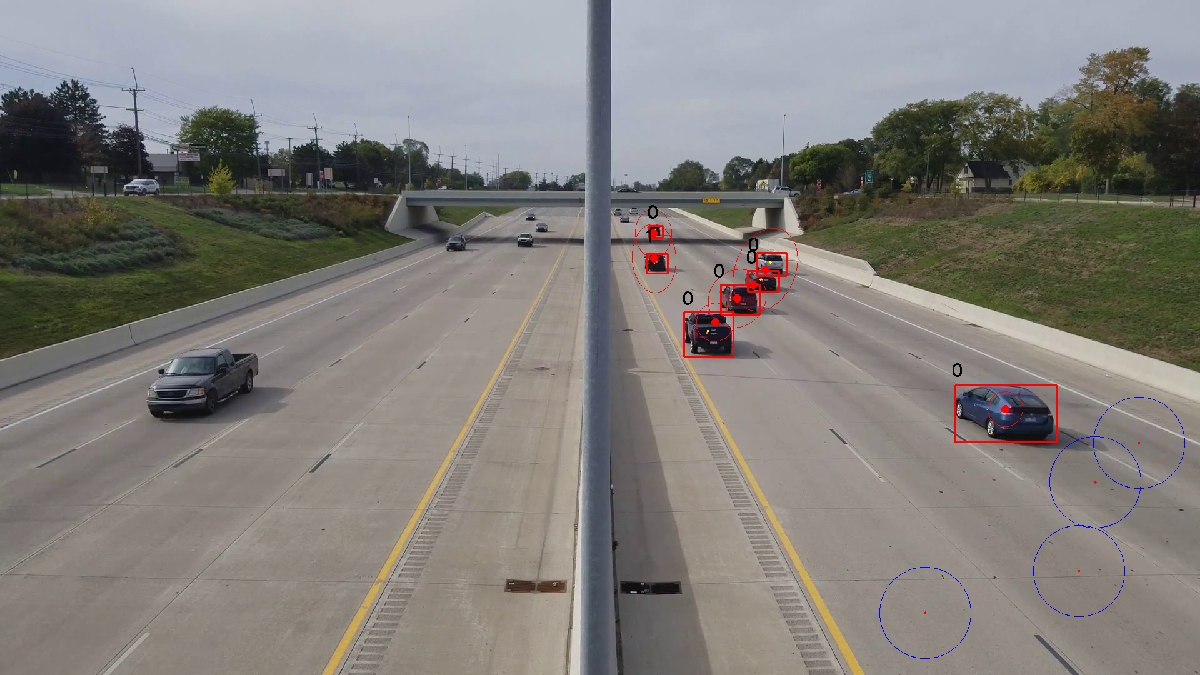
\includegraphics[width=\linewidth]{../../../experiments/E1/V1/SAM/78}
        \caption{Frame number: 78.}
        \label{fig:E1-V1-S2:08}
    \end{subfigure}
    \caption{Image sequence of tracked objects using the GM-PHD filter with the dynamic detection probability, the YOLO
    object detector and the SAM image segmentation model.}
    \label{fig:E1-V1-S2}
\end{figure}


\subsubsection{S3 -- Grounded SAM}
The experiment with settings \textit{S3} uses Grounding DINO object detector and the SAM image segmentation model.
All used parameters are included in Table \ref{tab:E1-V1-S3}.
\begin{table}[H]
    \centering
    \begin{tabular}{|c|c|c|c|c|c|c|c|c|c|}
        \hline
        $P_{D,k}(x)$ & $P$ & $\sigma_{\upsilon}$ & $\sigma_{\epsilon}$ & $T_H$ & $T_d$ & $T_p$ & $T_l$ & $T_{text}$ & $T_{bbox}$\\ \noalign{\hrule
        height 1.5pt}
        0.3 & $\diag(600,600,600,600)$ & 0.1 & 150 & 1 & 3 & 0.1 & 0.01 & 0.3 & 0.3\\
        \hline
    \end{tabular}
    \caption{The parameter settings for Experiment E1-V1-S3 with the dynamic detection probability.}
    \label{tab:E1-V1-S3}
\end{table}

Figure \ref{fig:E1-V1-S3} shows the performance of the GM-PHD filter with the dynamic detection probability with settings \textit{S3}.
\begin{itemize}
    \item \textbf{\ref{fig:E1-V1-S3:01}:} The utilization of a distinct object detection model results in an
    increased number of cars detected within the scene. However, only the four cars in the front have driven through
    the spawn
    points thus are considered within the true count.
    \item \textbf{\ref{fig:E1-V1-S3:02}:} All targets are effectively tracked without any issues.
    \item \textbf{\ref{fig:E1-V1-S3:03}:} Unlike YOLO, Grounding DINO successfully detects the arrival of a new car.
    \item In \textbf{\ref{fig:E1-V1-S3:04}, \ref{fig:E1-V1-S3:05}, \ref{fig:E1-V1-S3:06}} no events of greater
    importance occur.
    \item \textbf{\ref{fig:E1-V1-S3:07}:} Subsequently, the following arriving car is promptly detected and initialized.
    \item \textbf{\ref{fig:E1-V1-S3:08}:} This frame presents new challenges. Given the decreased distance between
    the cars and their proximity to each other, coupled with the model's ability to detect all of the cars, an excess of
    new
    targets emerges. To address this issue, adjustments to the motion noise are necessary. Additionally, for
    such scenarios, the implementation of the dynamic motion noise and the observation noise could offer a viable
    solution.
\end{itemize}

Figure \ref{gr:E1-V1-S3} shows, that the number of detected objects is far beyond the true count. Nevertheless,
the number of displayed targets is almost on spot till the frame 66. As the targets get closer to each
other, the
number of targets grows rapidly, causing errors to the number of tracked objects.

This setting outperforms the other settings. The performance of Grounding DINO brings another problems arising from
characteristics of the video. The video is taken from an angle, which makes the cars smaller as they carry on. These
dynamics align poorly with the static motion and the observation noise.

\begin{figure}[H]
    \centering
    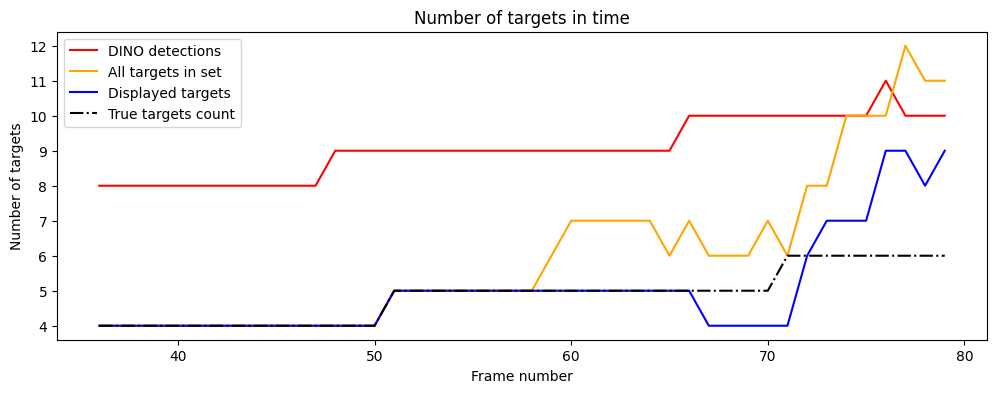
\includegraphics[width=\linewidth]{../../../experiments/E1/V1/DINO/dino_det}
    \caption{Development chart of the number of detected targets, targets in the filter's queue, displayed targets
    and the
    true
    targets' count.}
    \label{gr:E1-V1-S3}
\end{figure}

\begin{figure}[H]
    \centering
    \begin{subfigure}{0.48\textwidth}
        \centering
        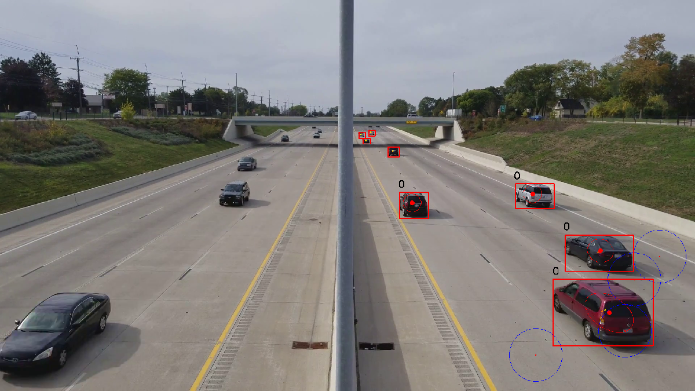
\includegraphics[width=\linewidth]{../../../experiments/E1/V1/DINO/36}
        \caption{Frame number: 36.}
        \label{fig:E1-V1-S3:01}
    \end{subfigure}
    \begin{subfigure}{0.48\textwidth}
        \centering
        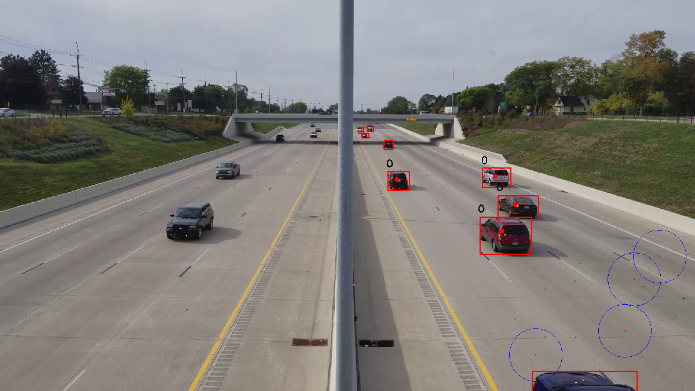
\includegraphics[width=\linewidth]{../../../experiments/E1/V1/DINO/48}
        \caption{Frame number: 48.}
        \label{fig:E1-V1-S3:02}
    \end{subfigure}
    \\
    \begin{subfigure}{0.48\textwidth}
        \centering
        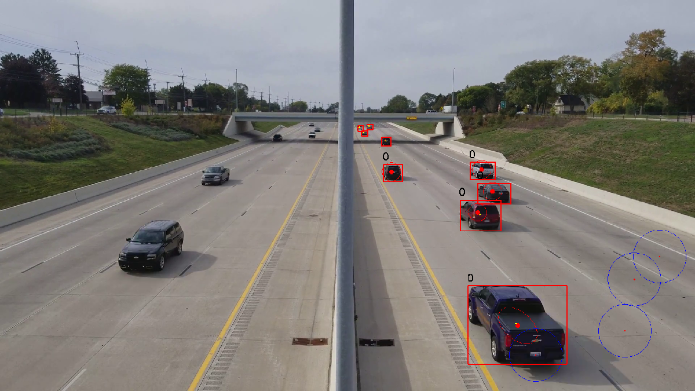
\includegraphics[width=\linewidth]{../../../experiments/E1/V1/DINO/54}
        \caption{Frame number: 54.}
        \label{fig:E1-V1-S3:03}
    \end{subfigure}
    \begin{subfigure}{0.48\textwidth}
        \centering
        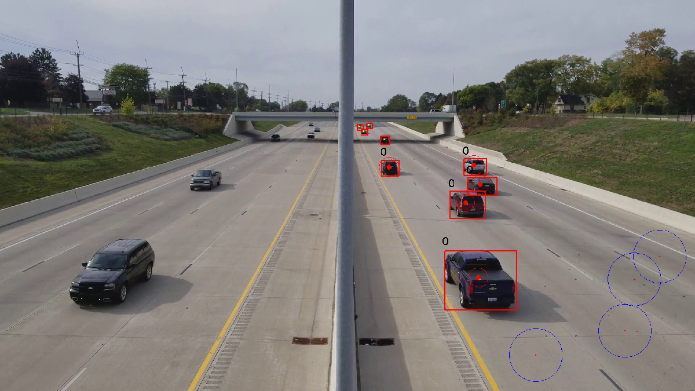
\includegraphics[width=\linewidth]{../../../experiments/E1/V1/DINO/58}
        \caption{Frame number: 58.}
        \label{fig:E1-V1-S3:04}
    \end{subfigure}
    \\
    \begin{subfigure}{0.48\textwidth}
        \centering
        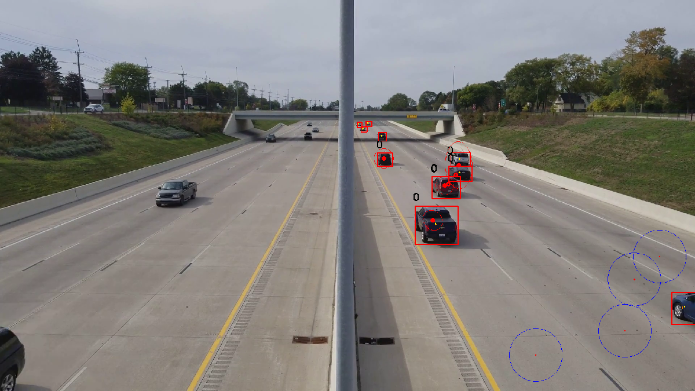
\includegraphics[width=\linewidth]{../../../experiments/E1/V1/DINO/67}
        \caption{Frame number: 67.}
        \label{fig:E1-V1-S3:05}
    \end{subfigure}
    \begin{subfigure}{0.48\textwidth}
        \centering
        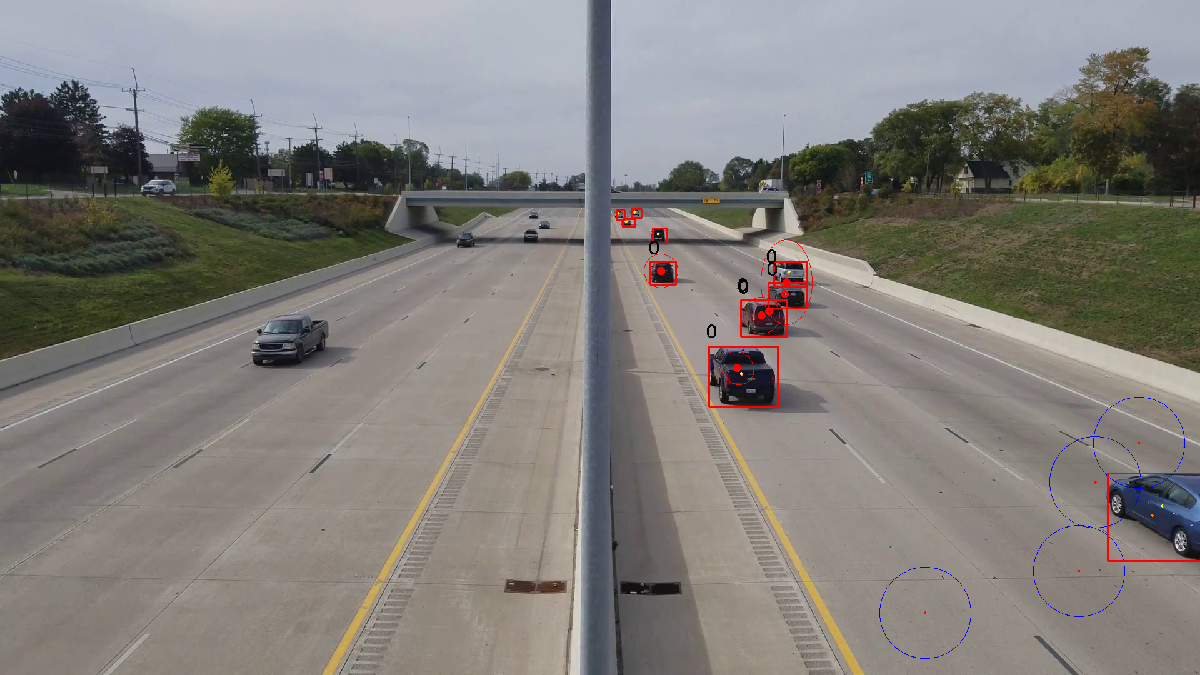
\includegraphics[width=\linewidth]{../../../experiments/E1/V1/DINO/69}
        \caption{Frame number: 69.}
        \label{fig:E1-V1-S3:06}
    \end{subfigure}
    \\
    \begin{subfigure}{0.48\textwidth}
        \centering
        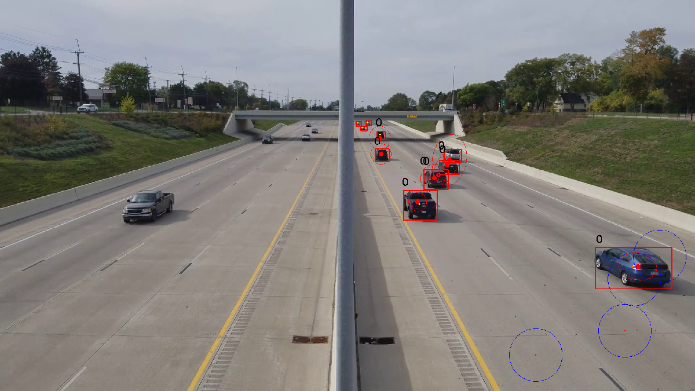
\includegraphics[width=\linewidth]{../../../experiments/E1/V1/DINO/73}
        \caption{Frame number: 73.}
        \label{fig:E1-V1-S3:07}
    \end{subfigure}
    \begin{subfigure}{0.48\textwidth}
        \centering
        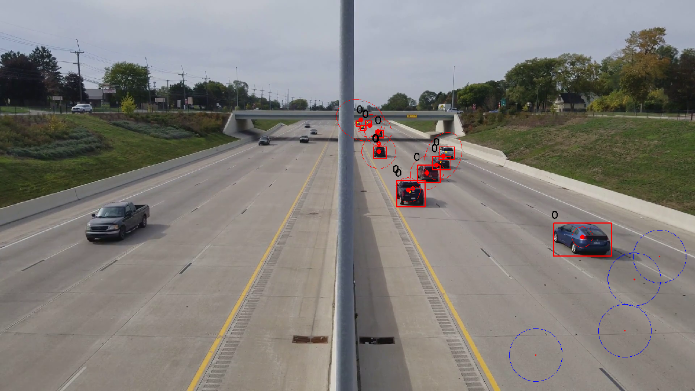
\includegraphics[width=\linewidth]{../../../experiments/E1/V1/DINO/78}
        \caption{Frame number: 79.}
        \label{fig:E1-V1-S3:08}
    \end{subfigure}
    \caption{Image sequence of tracked objects using the GM-PHD filter with the dynamic detection probability and
    the
    Grounded SAM model.}
    \label{fig:E1-V1-S3}
\end{figure}

\subsection{V2}
Video \textit{V2} is recorded at 29 fps. Only the cars driving from the left to the right are detected and tracked. In
the following
experiments
frames 83-109 of the
video \textit{V2} are
analyzed.
\subsection{V2 -- GM-PHD with the constant detection probability}
The measurements for the GM-PHD filter with the constant detection probability are obtained by the YOLO object detection
model. The parameters' values are displayed in Table \ref{tab:E1-V2-S0}.
\begin{table}[!h]
    \centering
    \begin{tabular}{|c|c|c|c|c|c|}
        \hline
        $P_{D}$ & $P$ & $\sigma_{\upsilon}$ & $\sigma_{\epsilon}$ & $T_p$ & $T_{YOLO}$ \\ \noalign{\hrule height 1.5pt}
        0.9 & $\diag(100,100,100,100)$ & 0.1 & 30 & 0.1 & 0.3\\
        \hline
    \end{tabular}
    \caption{The parameter settings for Experiment E1-V2 with the constant detection probability.}
    \label{tab:E1-V2-S0}
\end{table}

Figure \ref{fig:E1-V2-S0} displays the performance of the GM-PHD filter with the constant detection probability.
\begin{itemize}
    \item \textbf{\ref{fig:E1-V2-S0:01}:} The sequence begins with the frame number 83, wherein four targets have
    already been initialized and successfully detected.
    \item \textbf{\ref{fig:E1-V2-S0:02}:} Notably, the objects appear relatively small in comparison to the overall
    frame size. This size discrepancy contributes to a phenomenon where targets in a close proximity share
    measurements, resulting in the appearance of additional targets in the scene.
    \item \textbf{\ref{fig:E1-V2-S0:03}:} Despite the YOLO model failing to detect the fourth car, the target persists within the tracking system.
    \item \textbf{\ref{fig:E1-V2-S0:04}:} The previously undetected car is successfully identified once more, and
    the tracking of the target continues. Additionally, another car approaches the spawning point.
    \item \textbf{\ref{fig:E1-V2-S0:05}:} Regrettably, the car within the spawning area remains undetected and
    has not survived, probably
    due to its weight being insufficient to ensure survival. Concurrently, the first car exits the scene.
    \item \textbf{\ref{fig:E1-V2-S0:06}:} Subsequently, the car at the spawning point is detected once again and remains sufficiently close to be initialized as a target. The scene concludes with four true objects and four accurately tracked targets.
\end{itemize}


The GM-PHD filter with the constant detection probability is accurate in scenarios, where the object detector does not
miss detections regularly. Figure \ref{gr:E1-V2-S0} shows that the number of displayed targets is close enough
to the true count. Even false detections created by YOLO did not mislead the filter.


\begin{figure}[H]
    \centering
    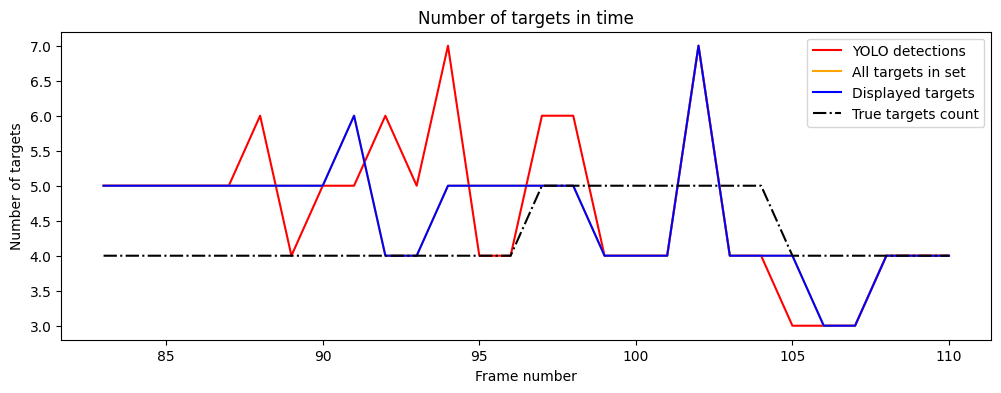
\includegraphics[width=\linewidth]{../../../experiments/E1/V2/noPd/staticPd_det}
    \caption{Development chart of the number of detected targets, targets in the filter's queue, displayed targets
    and the
    true
    targets' count.}
    \label{gr:E1-V2-S0}
\end{figure}

\begin{figure}[H]
    \centering
    \begin{subfigure}{0.48\textwidth}
        \centering
        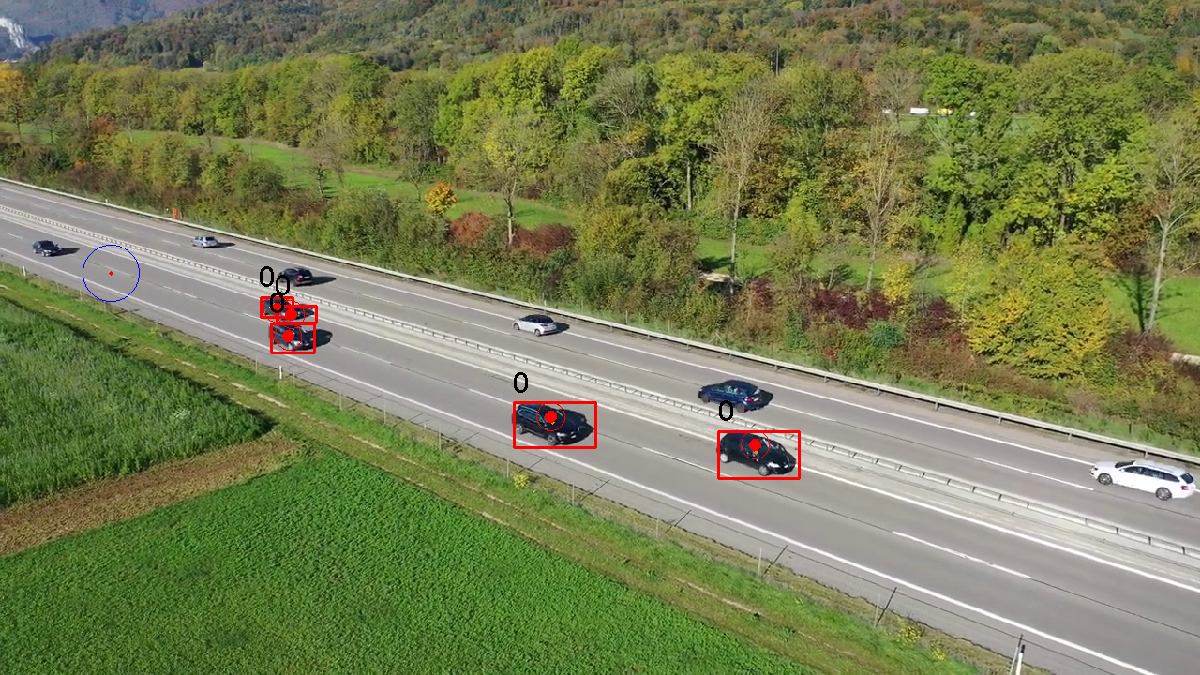
\includegraphics[width=\linewidth]{../../../experiments/E1/V2/noPd/83}
        \caption{Frame number: 83.}
        \label{fig:E1-V2-S0:01}
    \end{subfigure}
    \begin{subfigure}{0.48\textwidth}
        \centering
        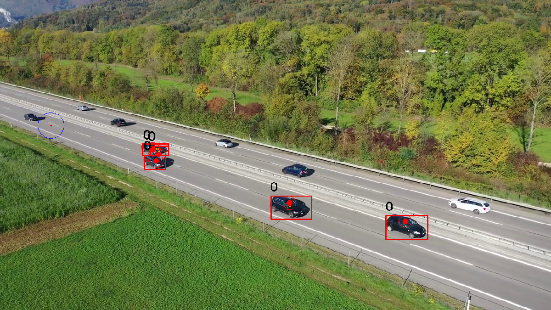
\includegraphics[width=\linewidth]{../../../experiments/E1/V2/noPd/90}
        \caption{Frame number: 90.}
        \label{fig:E1-V2-S0:02}
    \end{subfigure}
    \\
    \begin{subfigure}{0.48\textwidth}
        \centering
        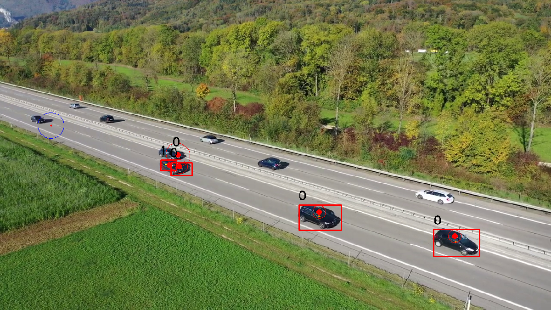
\includegraphics[width=\linewidth]{../../../experiments/E1/V2/noPd/95}
        \caption{Frame number: 95.}
        \label{fig:E1-V2-S0:03}
    \end{subfigure}
    \begin{subfigure}{0.48\textwidth}
        \centering
        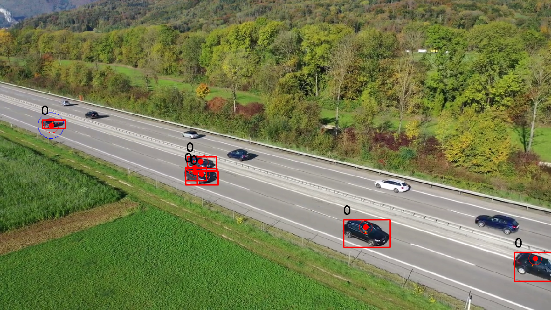
\includegraphics[width=\linewidth]{../../../experiments/E1/V2/noPd/102}
        \caption{Frame number: 102.}
        \label{fig:E1-V2-S0:04}
    \end{subfigure}
    \\
    \begin{subfigure}{0.48\textwidth}
        \centering
        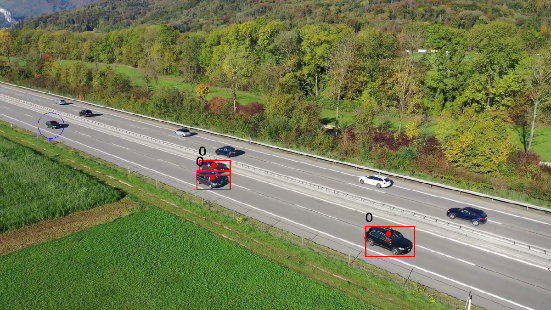
\includegraphics[width=\linewidth]{../../../experiments/E1/V2/noPd/105}
        \caption{Frame number: 105.}
        \label{fig:E1-V2-S0:05}
    \end{subfigure}
    \begin{subfigure}{0.48\textwidth}
        \centering
        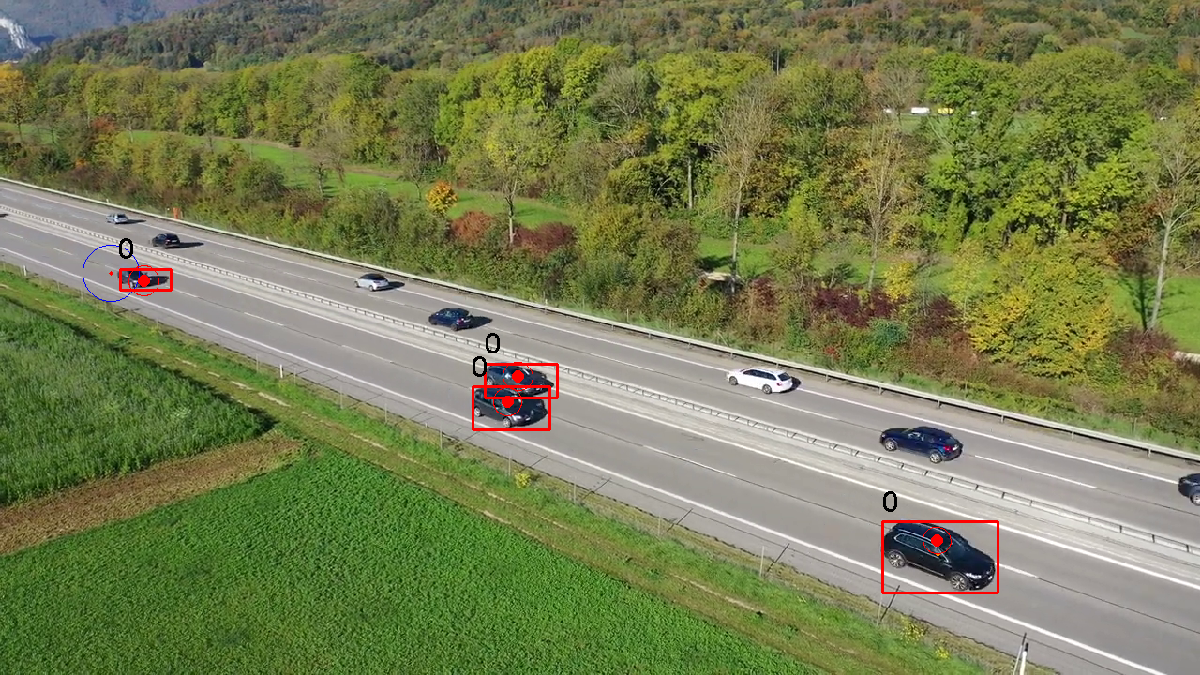
\includegraphics[width=\linewidth]{../../../experiments/E1/V2/noPd/110}
        \caption{Frame number: 110.}
        \label{fig:E1-V2-S0:06}
    \end{subfigure}
    \caption{Image sequence of tracked objects using the GM-PHD filter with the constant detection probability.}
    \label{fig:E1-V2-S0}
\end{figure}


\subsection{V2 -- GM-PHD with the dynamic detection probability}
Experiments carried out on the video \textit{V2} using the GM-PHD filter with the dynamic detection probability and
different
settings
are
demonstrated in following sections.
\subsubsection{S1 -- YOLO + YOLO}
This experiment uses settings \textit{S1}, where the YOLO model provides both object detection bboxes and
segmentation masks.
The parameter settings are shown in Table \ref{tab:E1-V2-S1}.
\begin{table}[H]
    \centering
    \begin{tabular}{|c|c|c|c|c|c|c|c|c|}
        \hline
        $P_{D,k}(x)$ & $P$ & $\sigma_{\upsilon}$ & $\sigma_{\epsilon}$ & $T_H$ & $T_d$ & $T_p$ & $T_l$ & $T_{YOLO}$ \\ \noalign{\hrule
        height 1.5pt}
        0.3 & $\diag(600,600,600,600)$ & 0.1 & 30 & 1 & 3 & 0.1 & 0.01 & 0.3\\
        \hline
    \end{tabular}
    \caption{The parameter settings for Experiment E1-V2-S1 with the dynamic detection probability.}
    \label{tab:E1-V2-S1}
\end{table}

Figure \ref{fig:E1-V2-S1} shows the performance of the GM-PHD filter with the dynamic detection probability with settings \textit{S1}.
\begin{itemize}
    \item \textbf{\ref{fig:E1-V2-S1:01}:} Analogously to the previous analysis, four targets have surpassed the
    spawning point and are tracked by the GM-PHD filter. The targets' presence in the close proximity results in an
    additional false targets' existence.
    \item \textbf{\ref{fig:E1-V2-S1:02}:} The problem of targets' neighboring persists.
    \item \textbf{\ref{fig:E1-V2-S1:03}:} Moreover, the YOLO model classifies the targets' shadows as another cars,
    causing the initialization of extra targets.
    \item \textbf{\ref{fig:E1-V2-S1:04}:} A new car crosses the spawning point, yet the YOLO model fails to detect it.
    \item \textbf{\ref{fig:E1-V2-S1:05}:} The new car has been previously detected and
    initialized. The two
    neighbouring cars still generate additional false targets.
    \item \textbf{\ref{fig:E1-V2-S1:06}:} Finally, there appear only two targets representing the two cars. The other
    two
    cars are tracked properly.
\end{itemize}

Figure \ref{gr:E1-V2-S1} depicts a similar performance of the GM-PHD filter with the dynamic detection probability as
the GM-PHD filter with the constant detection probability. The number of displayed targets exceeds the true number of
targets due to already presented reasons.


The improved ability of the target's survival resulted in a slightly decreased the overall tracking performance. The
YOLO model
has been able to detect tracked objects flawlessly, which leads to needlessness of the dynamic detection
probability
and modified pruning method enabling enhanced targets' ability to survive.

However, the goal of this experiment is to examine the tracking capability of the GM-PHD filter with the proposed
dynamic
detection probability in common flawless scenarios. This experiment verifies the method to be sufficient.

\begin{figure}[H]
    \centering
    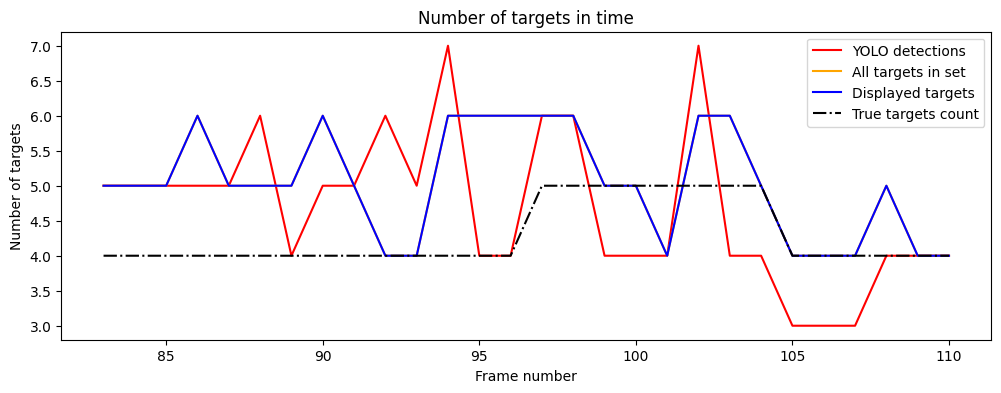
\includegraphics[width=\linewidth]{../../../experiments/E1/V2/YOLO/yolo_det}
    \caption{Development chart of the number of detected targets, targets in the filter's queue, displayed targets
    and the
    true targets' count.}
    \label{gr:E1-V2-S1}
\end{figure}

\begin{figure}[H]
    \centering
    \begin{subfigure}{0.48\textwidth}
        \centering
        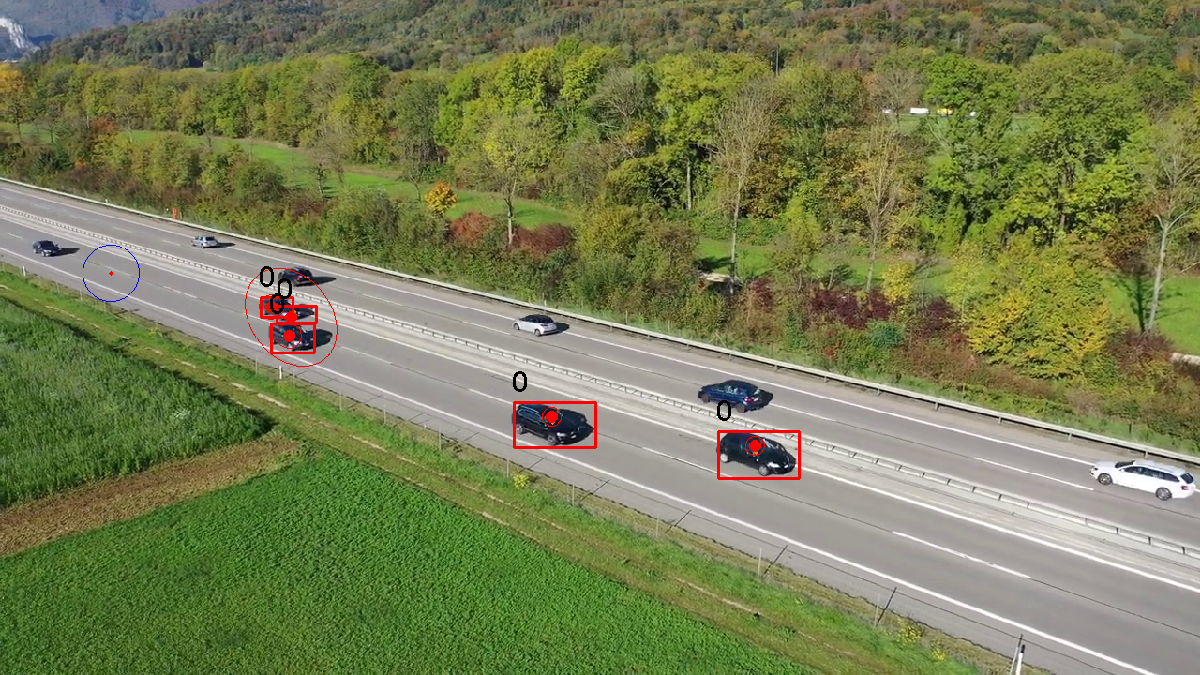
\includegraphics[width=\linewidth]{../../../experiments/E1/V2/YOLO/83}
        \caption{Frame number: 83.}
        \label{fig:E1-V2-S1:01}
    \end{subfigure}
    \begin{subfigure}{0.48\textwidth}
        \centering
        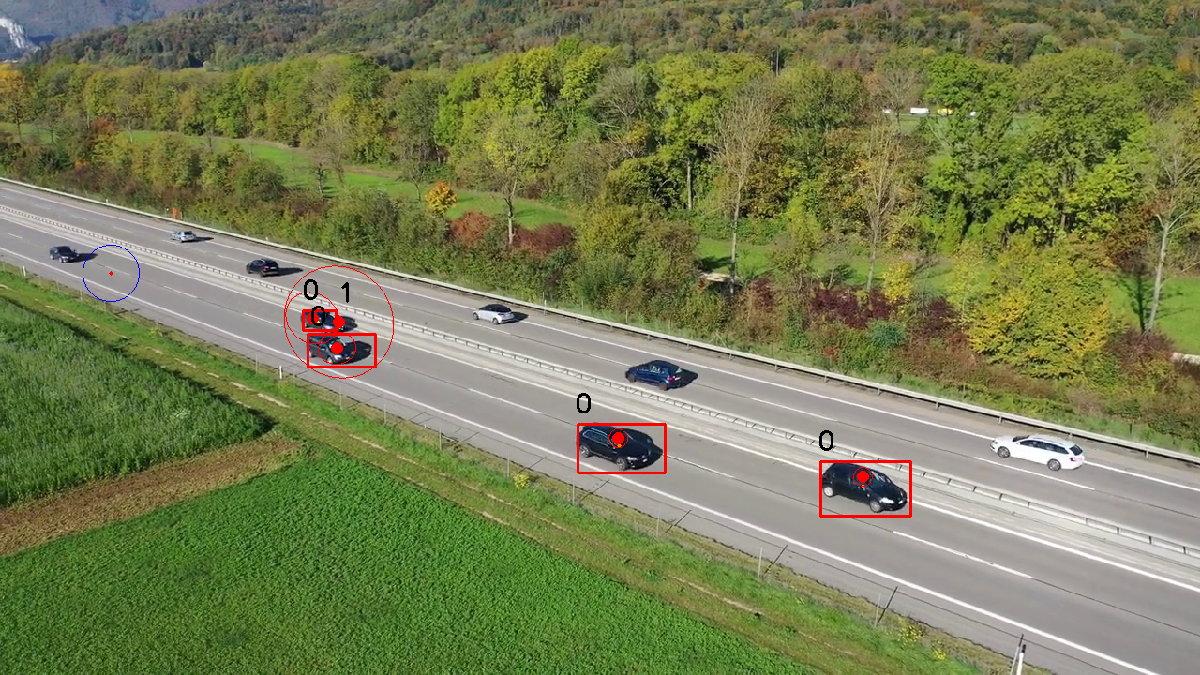
\includegraphics[width=\linewidth]{../../../experiments/E1/V2/YOLO/89}
        \caption{Frame number: 89.}
        \label{fig:E1-V2-S1:02}
    \end{subfigure}
    \\
    \begin{subfigure}{0.48\textwidth}
        \centering
        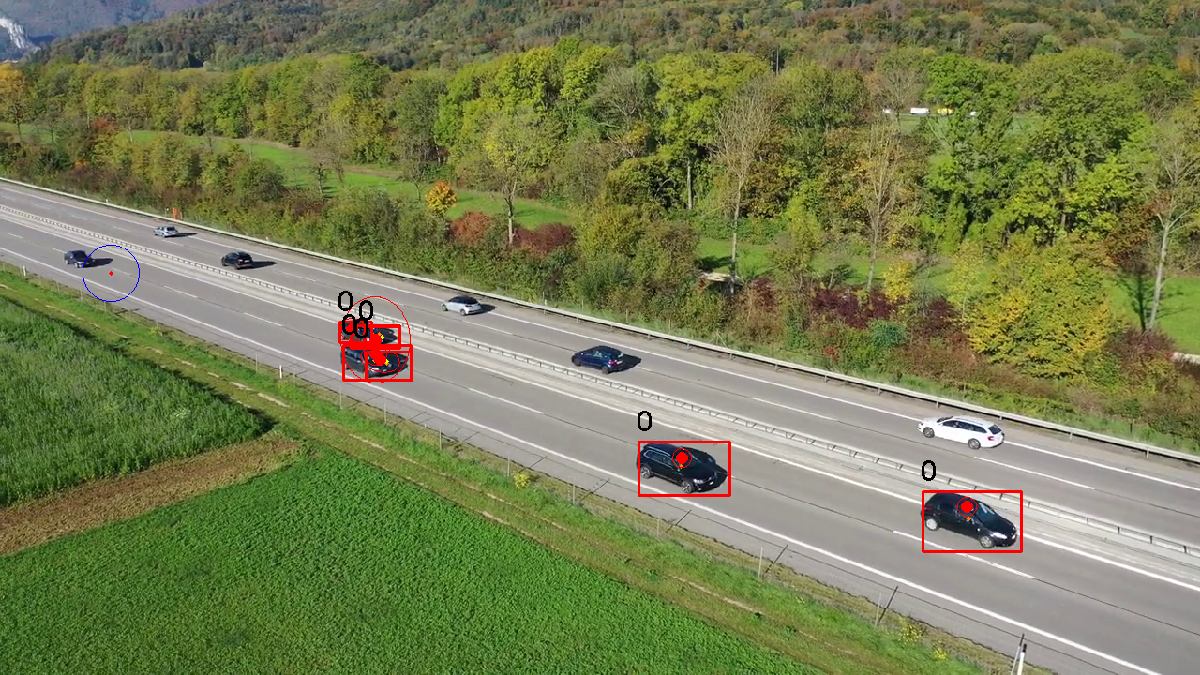
\includegraphics[width=\linewidth]{../../../experiments/E1/V2/YOLO/94}
        \caption{Frame number: 94.}
        \label{fig:E1-V2-S1:03}
    \end{subfigure}
    \begin{subfigure}{0.48\textwidth}
        \centering
        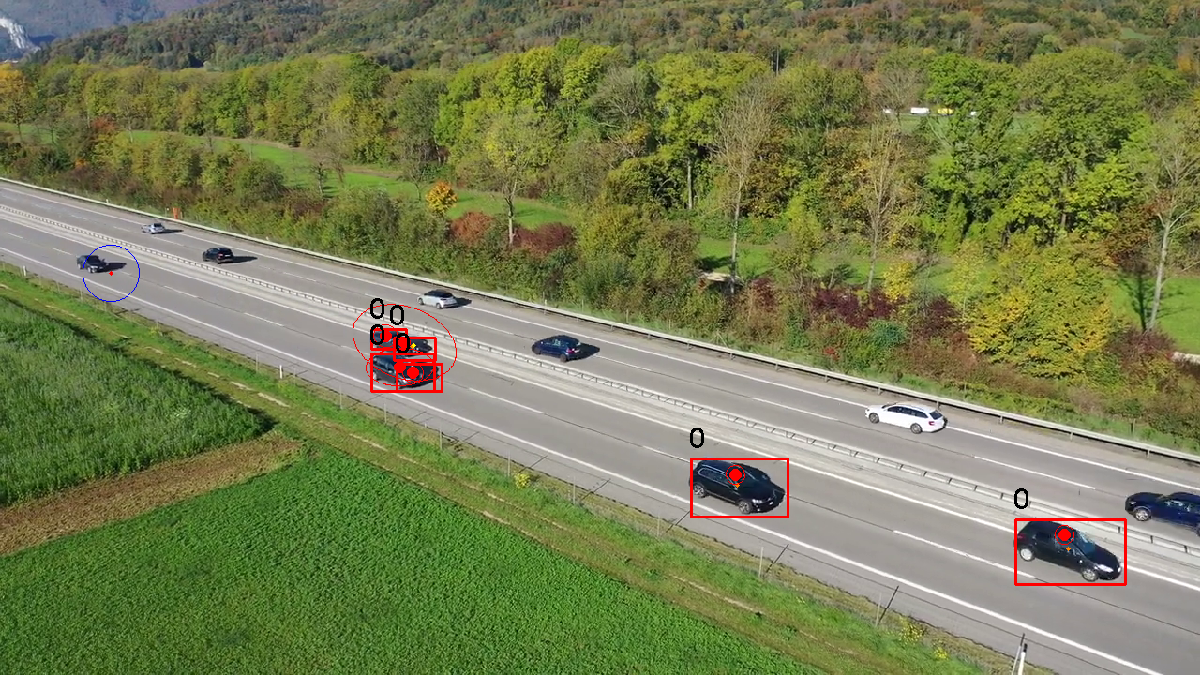
\includegraphics[width=\linewidth]{../../../experiments/E1/V2/YOLO/98}
        \caption{Frame number: 98.}
        \label{fig:E1-V2-S1:04}
    \end{subfigure}
    \\
    \begin{subfigure}{0.48\textwidth}
        \centering
        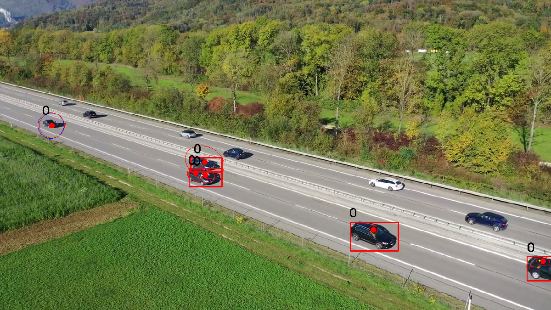
\includegraphics[width=\linewidth]{../../../experiments/E1/V2/YOLO/103}
        \caption{Frame number: 103.}
        \label{fig:E1-V2-S1:05}
    \end{subfigure}
    \begin{subfigure}{0.48\textwidth}
        \centering
        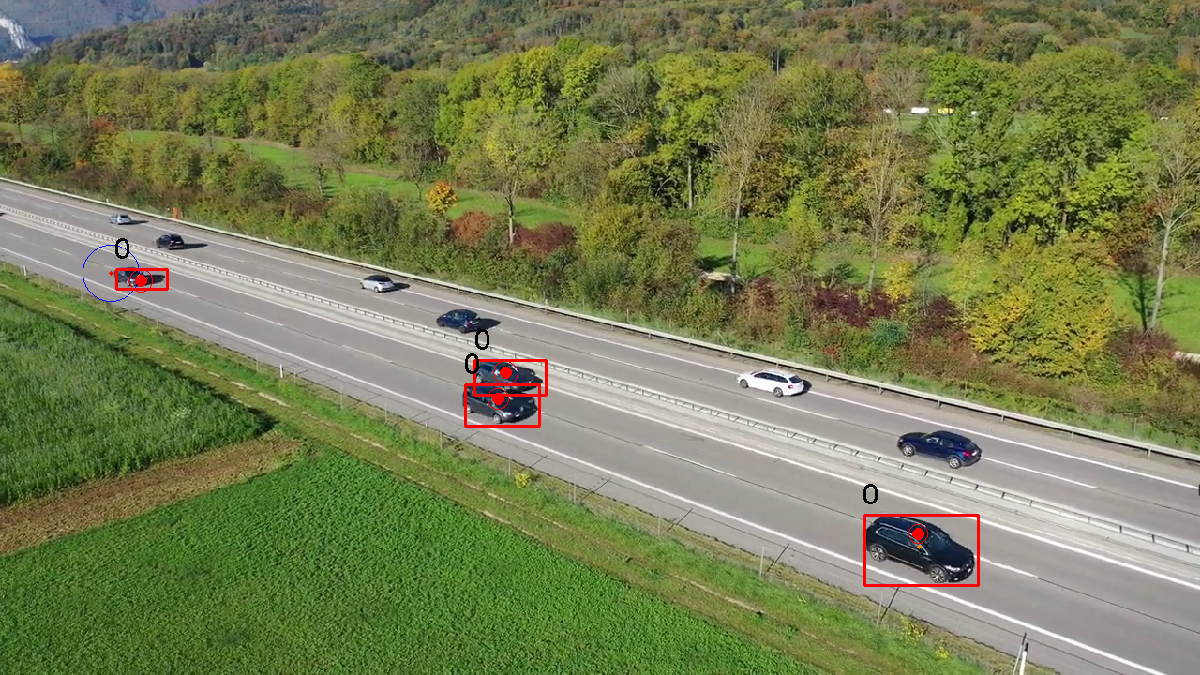
\includegraphics[width=\linewidth]{../../../experiments/E1/V2/YOLO/109}
        \caption{Frame number: 109.}
        \label{fig:E1-V2-S1:06}
    \end{subfigure}
    \caption{Image sequence of tracked objects using the GM-PHD filter with the dynamic detection probability and YOLO
    only.}
    \label{fig:E1-V2-S1}
\end{figure}





\subsubsection{S2 -- YOLO + SAM}
As in experiment \textit{E1}, the next settings employs \textit{S2} with the YOLO object detector and the SAM
segmentation model.
All parameters are included in Table \ref{tab:E1-V2-S2}.
\begin{table}[H]
    \centering
    \begin{tabular}{|c|c|c|c|c|c|c|c|c|}
        \hline
        $P_{D,k}(x)$ & $P$ & $\sigma_{\upsilon}$ & $\sigma_{\epsilon}$ & $T_H$ & $T_d$ & $T_p$ & $T_l$ & $T_{YOLO}$ \\ \noalign{\hrule
        height 1.5pt}
        0.3 & $\diag(100,100,100,100)$ & 0.1 & 30 & 1 & 3 & 0.1 & 0.01 & 0.3\\
        \hline
    \end{tabular}
    \caption{The parameter settings for Experiment E1-V2-S2 with the dynamic detection probability.}
    \label{tab:E1-V2-S2}
\end{table}


The situation resembles the situation with settings \textit{S1}. Four targets occur in Figure \ref{fig:E1-V2-S2:01}.
They continue in their path while all targets are tracked successfully with one exception. No additional targets appear
in the subsequent frames. The YOLO model detects a car's shadow and clasifies it as an another car, which makes
the added target in Figure \ref{fig:E1-V2-S2:03}. Due to the merging step, this false target does not survive to the subsequent
frames. A new car is initialized in Figure \ref{fig:E1-V2-S2:04}. All targets are tracked in the
last frames.

The number of displayed targets is close to the true number of targets in Figure
\ref{gr:E1-V2-S2}. The number of
detected targets exceeds the number of true targets for majority of the time, due to the presence of false
detections.

Settings \textit{S2} exhibit a slight improvement over settings \textit{S1}, which is reflected in the reduced error
between the number of displayed targets and the true count.

\begin{figure}[H]
    \centering
    \includegraphics[width=\linewidth]{../../../experiments/E1/V2/SAM/sam_det}
    \caption{Development chart of the number of detected targets, targets in the filter's queue, displayed targets and
    true targets' count.}
    \label{gr:E1-V2-S2}
\end{figure}

\begin{figure}[H]
    \centering
    \begin{subfigure}{0.48\textwidth}
        \centering
        \includegraphics[width=\linewidth]{../../../experiments/E1/V2/SAM/83}
        \caption{Frame number: 83.}
        \label{fig:E1-V2-S2:01}
    \end{subfigure}
    \begin{subfigure}{0.48\textwidth}
        \centering
        \includegraphics[width=\linewidth]{../../../experiments/E1/V2/SAM/89}
        \caption{Frame number: 89.}
        \label{fig:E1-V2-S2:02}
    \end{subfigure}
    \\
    \begin{subfigure}{0.48\textwidth}
        \centering
        \includegraphics[width=\linewidth]{../../../experiments/E1/V2/SAM/94}
        \caption{Frame number: 94.}
        \label{fig:E1-V2-S2:03}
    \end{subfigure}
    \begin{subfigure}{0.48\textwidth}
        \centering
        \includegraphics[width=\linewidth]{../../../experiments/E1/V2/SAM/98}
        \caption{Frame number: 98.}
        \label{fig:E1-V2-S2:04}
    \end{subfigure}
    \\
    \begin{subfigure}{0.48\textwidth}
        \centering
        \includegraphics[width=\linewidth]{../../../experiments/E1/V2/SAM/103}
        \caption{Frame number: 103.}
        \label{fig:E1-V2-S2:05}
    \end{subfigure}
    \begin{subfigure}{0.48\textwidth}
        \centering
        \includegraphics[width=\linewidth]{../../../experiments/E1/V2/SAM/109}
        \caption{Frame number: 109.}
        \label{fig:E1-V2-S2:06}
    \end{subfigure}
    \caption{Image sequence of tracked objects using the GM-PHD filter with the dynamic detection probability, the YOLO
    object detector and the SAM image segmentation model.}
    \label{fig:E1-V2-S2}
\end{figure}


\subsubsection{S3 -- Grounded SAM}
The combination of Grounding DINO and SAM is tested using the video \textit{V2} as well. Used parameteres are given in
Table \ref{tab:E1-V2-S3}.
\begin{table}[H]
    \centering
    \begin{tabular}{|c|c|c|c|c|c|c|c|c|c|}
        \hline
        $P_{D,k}(x)$ & $P$ & $\sigma_{\upsilon}$ & $\sigma_{\epsilon}$ & $T_H$ & $T_d$ & $T_p$ & $T_l$ & $T_{text}$ & $T_{bbox}$\\ \noalign{\hrule
        height 1.5pt}
        0.3 & $\diag(100,100,100,100)$ & 0.1 & 30 & 1 & 3 & 0.1 & 0.01 & 0.3 & 0.3\\
        \hline
    \end{tabular}
    \caption{The parameter settings for Experiment E1-V2-S3 with the dynamic detection probability.}
    \label{tab:E1-V2-S3}
\end{table}

Figure \ref{fig:E1-V2-S3} reveals a better object detection. As a result, the tracking of objects is more precise than
in the other settings.
\begin{itemize}
    \item \textbf{\ref{fig:E1-V2-S3:01}:} Starting with four tracked targets in the frame no. 83.
    \item \textbf{\ref{fig:E1-V2-S3:02}:} As in Experiment E1-V1, the motion and observation noise covariances
    seem to be too large for this scenario. The third and the fourth car's measurement reaches the validation region of
    each other. This situation creates new undesired targets.
    \item \textbf{\ref{fig:E1-V2-S3:03}:} The exact same situation happens in this frame.
    \item \textbf{\ref{fig:E1-V2-S3:04}:} Another car reaches the spawning point.
    \item \textbf{\ref{fig:E1-V2-S3:05}:} Five targets appear in the scene, all of them correctly tracked.
    \item \textbf{\ref{fig:E1-V2-S3:06}:} The scenario ends with four properly detected and tracked objects.
\end{itemize}

Even though the two cars driving side by side cause the filter with given parameters a few modest problems, the merging
and
the pruning steps can usually deal with such situations, as seen in Figure \ref{gr:E1-V2-S3}. The line
showing
the number of displayed targets almost copies the line showing the true counts. The graph also shows the problem of
two neighbouring targets and the problem of false detections. The peaks in the red line show these false detections,
the filter remains unaffected and holds the true number of targets.


As in Experiment \textit{E1-V1}, this setting outperform the other settings variations. Moreover, due to the more
precise
object detection, the filter is able to deal with problems such as two targets appearing in the same neighbourhood or
false
detections. However, settings \textit{S3} is very sensitive to motion and observation noise parametrization, thus
these covariance matrices have to be set carefully.

\begin{figure}[H]
    \centering
    \includegraphics[width=\linewidth]{../../../experiments/E1/V2/DINO/dino_det}
    \caption{Development chart of the number of detected targets, targets in the filter's queue, displayed targets and
    true targets' count.}
    \label{gr:E1-V2-S3}
\end{figure}

\begin{figure}[H]
    \centering
    \begin{subfigure}{0.48\textwidth}
        \centering
        \includegraphics[width=\linewidth]{../../../experiments/E1/V2/DINO/83}
        \caption{Frame number: 83.}
        \label{fig:E1-V2-S3:01}
    \end{subfigure}
    \begin{subfigure}{0.48\textwidth}
        \centering
        \includegraphics[width=\linewidth]{../../../experiments/E1/V2/DINO/89}
        \caption{Frame number: 89.}
        \label{fig:E1-V2-S3:02}
    \end{subfigure}
    \\
    \begin{subfigure}{0.48\textwidth}
        \centering
        \includegraphics[width=\linewidth]{../../../experiments/E1/V2/DINO/94}
        \caption{Frame number: 94.}
        \label{fig:E1-V2-S3:03}
    \end{subfigure}
    \begin{subfigure}{0.48\textwidth}
        \centering
        \includegraphics[width=\linewidth]{../../../experiments/E1/V2/DINO/98}
        \caption{Frame number: 98.}
        \label{fig:E1-V2-S3:04}
    \end{subfigure}
    \\
    \begin{subfigure}{0.48\textwidth}
        \centering
        \includegraphics[width=\linewidth]{../../../experiments/E1/V2/DINO/103}
        \caption{Frame number: 103.}
        \label{fig:E1-V2-S3:05}
    \end{subfigure}
    \begin{subfigure}{0.48\textwidth}
        \centering
        \includegraphics[width=\linewidth]{../../../experiments/E1/V2/DINO/109}
        \caption{Frame number: 109.}
        \label{fig:E1-V2-S3:06}
    \end{subfigure}
    \caption{Image sequence of tracked objects using the GM-PHD filter with the dynamic detection probability, the DINO
    object detector and the SAM image segmentation model.}
    \label{fig:E1-V2-S3}
\end{figure}

\section{E2: Traffic with an obstacle}
\newcommand{\Ex}{E2}
The previous experiment demonstrated the performance of our proposed GM-PHD filter method, which incorporated
the dynamic detection probability and the modified pruning. Our method has proven superior to the standard
GM-PHD
filter with the constant
detection probability. Nevertheless, our method was primarily designed to excel in situations where obstacles obscure camera views. To assess its effectiveness in such scenarios, we propose Experiment \textit{E2}.

\subsection{V3}
\newcommand{\Vs}{V3}
In the video \textit{V3} a light pole is in the camera's view, preventing the object detector to detect hidden objects. The
frame rate of this video is set to 10 fps.

\subsection{V3 - GM-PHD with the constant detection probability}
\newcommand{\Set}{S0}
The targets cannot persist beyond a certain number of time steps without being measured, resulting in their loss once they surpass an obstacle. To avert a permanent loss, a new spawning point is introduced immediately after the obstacle to revive the lost target. However, this approach comes with a drawback: the revived target starts afresh without retaining its previous history.

Parameter settings are embodied in Table \ref{tab:\Ex-\Vs-\Set}.

\begin{table}[!h]
    \centering
    \begin{tabular}{|c|c|c|c|c|c|}
        \hline
        $P_{D}$ & $P$ & $\sigma_{\upsilon}$ & $\sigma_{\epsilon}$ & $T_p$ & $T_{YOLO}$ \\ \noalign{\hrule height 1.5pt}
        0.9 & $diag(500,500,500,500)$ & 0.1 & 100 & 0.1 & 0.3\\
        \hline
    \end{tabular}
    \caption{The parameter settings for Experiment {\Ex-\Vs} with the constant detection probability.}
    \label{tab:\Ex-\Vs-\Set}
\end{table}

Figure \ref{fig:\Ex-\Vs-\Set} shows some highlights of the GM-PHD filter with the constant detection probability.
\begin{itemize}
    \item \textbf{\ref{fig:\Ex-\Vs-\Set:01}:} The sequence starts with the frame no. 7. The first car is initiaized by
    the spawning point.
    \item \textbf{\ref{fig:\Ex-\Vs-\Set:02}:} The first car arrives to an obstacle. Meanwhile, the second car arrives.
    \item \textbf{\ref{fig:\Ex-\Vs-\Set:03}:} The YOLO object detector is not able to detect the hidden car. The target is removed.
    \item \textbf{\ref{fig:\Ex-\Vs-\Set:04}:} The previously lost target is detected and initialized due to the
    second spawning point. Nevertheless, the history of this target is still lost. Moreover, the target has not been tracked for five consecutive frames.
    \item \textbf{\ref{fig:\Ex-\Vs-\Set:05}:} The second car is not detected due to the obstacle. The track of the target is lost.
    \item \textbf{\ref{fig:\Ex-\Vs-\Set:06}:} The target is once again initialized by the second spawning point. The
    third car approaches the first spawning point.
    \item \textbf{\ref{fig:\Ex-\Vs-\Set:07}:} The last car is also not detected behind the obstacle, thus its track is lost.
    \item \textbf{\ref{fig:\Ex-\Vs-\Set:08}:} Even though the target is reborn, the track of this target has not been
    available for 6 frames in a row. The other two cars are further away and appear to be in the same neighbourhood.
    The filter merged these two targets into a single one.
\end{itemize}

According to Graph \ref{gr:\Ex-\Vs-\Set}, the filter is able to track the targets admirably. However, the graph also
shows the weakness of this approach. The peaks displaying the target's loss are clearly present.

With the second spawn point enabling targets to reborn, the GM-PHD filter is able to track all the targets accurately.
The weakness of this approach is definite -- if a target is reborn, it is a whole new target without any history.

\begin{figure}[H]
    \centering
    \includegraphics[width=\linewidth]{../../../experiments/\Ex/\Vs/noPd/staticPd_det}
    \caption{Development chart of the number of detected targets, targets in the filter's queue, displayed targets and
    true targets' count.}
    \label{gr:\Ex-\Vs-\Set}
\end{figure}

\begin{figure}[H]
    \centering
    \begin{subfigure}{0.23\textwidth}
        \centering
        \includegraphics[width=\linewidth]{../../../experiments/\Ex/\Vs/noPd/7}
        \caption{Frame number: 7.}
        \label{fig:\Ex-\Vs-\Set:01}
    \end{subfigure}
    \begin{subfigure}{0.23\textwidth}
        \centering
        \includegraphics[width=\linewidth]{../../../experiments/\Ex/\Vs/noPd/33}
        \caption{Frame number: 33.}
        \label{fig:\Ex-\Vs-\Set:02}
    \end{subfigure}
    \begin{subfigure}{0.23\textwidth}
        \centering
        \includegraphics[width=\linewidth]{../../../experiments/\Ex/\Vs/noPd/38}
        \caption{Frame number: 38.}
        \label{fig:\Ex-\Vs-\Set:03}
    \end{subfigure}
    \begin{subfigure}{0.23\textwidth}
        \centering
        \includegraphics[width=\linewidth]{../../../experiments/\Ex/\Vs/noPd/43}
        \caption{Frame number: 43.}
        \label{fig:\Ex-\Vs-\Set:04}
    \end{subfigure}
    \\
    \begin{subfigure}{0.23\textwidth}
        \centering
        \includegraphics[width=\linewidth]{../../../experiments/\Ex/\Vs/noPd/55}
        \caption{Frame number: 55.}
        \label{fig:\Ex-\Vs-\Set:05}
    \end{subfigure}
    \begin{subfigure}{0.23\textwidth}
        \centering
        \includegraphics[width=\linewidth]{../../../experiments/\Ex/\Vs/noPd/60}
        \caption{Frame number: 60.}
        \label{fig:\Ex-\Vs-\Set:06}
    \end{subfigure}
    \begin{subfigure}{0.23\textwidth}
        \centering
        \includegraphics[width=\linewidth]{../../../experiments/\Ex/\Vs/noPd/85}
        \caption{Frame number: 85.}
        \label{fig:\Ex-\Vs-\Set:07}
    \end{subfigure}
    \begin{subfigure}{0.23\textwidth}
        \centering
        \includegraphics[width=\linewidth]{../../../experiments/\Ex/\Vs/noPd/92}
        \caption{Frame number: 92.}
        \label{fig:\Ex-\Vs-\Set:08}
    \end{subfigure}
    \caption{Image sequence of tracked objects using the GM-PHD filter with the constant detection probability.}
    \label{fig:\Ex-\Vs-\Set}
\end{figure}




\subsection{V3 -- GM-PHD with the dynamic detection probability}
Experiments using the video \textit{V3} utilizing the GM-PHD filter with the dynamic detection probability and
settings \textit{S1, S2,
    S3} are
demonstrated in following sections.
\subsubsection{S1 -- YOLO + YOLO}
\renewcommand{\Set}{S1}
This experiment uses settings \textit{S1}, where the YOLO model provides both object detection bboxes and
segmentation masks.
The parameter settings are shown in Table \ref{tab:\Ex-\Vs-\Set}.
\begin{table}[H]
    \centering
    \begin{tabular}{|c|c|c|c|c|c|c|c|c|}
        \hline
        $P_{D,k}(x)$ & $P$ & $\sigma_{\upsilon}$ & $\sigma_{\epsilon}$ & $T_H$ & $T_d$ & $T_p$ & $T_l$ & $T_{YOLO}$ \\ \noalign{\hrule
        height 1.5pt}
        0.3 & $diag(500,500,500,500)$ & 0.1 & 100 & 2 & 3 & 0.1 & 0.0001 & 0.3\\
        \hline
    \end{tabular}
    \caption{The parameter settings for Experiment {\Ex-\Vs-\Set} with the dynamic detection probability.}
    \label{tab:\Ex-\Vs-\Set}
\end{table}

Figure \ref{fig:\Ex-\Vs-\Set} shows the performance of the GM-PHD filter with the dynamic detection probability with settings \textit{S1}.
\begin{itemize}
    \item \textbf{\ref{fig:\Ex-\Vs-\Set:01}:} The tracking starts with frame no. 7. The first target approaches the spawning point.
    \item \textbf{\ref{fig:\Ex-\Vs-\Set:02}:} The first car reaches the light pole. The second car appears in the scene.
    \item \textbf{\ref{fig:\Ex-\Vs-\Set:03}:} The first car is detected by YOLO for the last time before
    temporarily disappearing
    behind the obstacle.
    \item \textbf{\ref{fig:\Ex-\Vs-\Set:04}:} Even though the first car has not been detected for 5 frames, it is able
    to survive without the second spawning point.
    \item \textbf{\ref{fig:\Ex-\Vs-\Set:05}:} In this frame, an example of the \textit{hidden} target's state can be
    seen. The second car is annotated with number 1, i.e., it is considered as hidden.
    \item \textbf{\ref{fig:\Ex-\Vs-\Set:06}:} The second car overcomes the obstacle and continues in its path. This target was able to survive for 6 consecutive time steps.
    \item \textbf{\ref{fig:\Ex-\Vs-\Set:07}:} As the two cars appear close to each other, more measurements appear in
    the validation region of the targets. The third car is not detected behind the light pole, but is still tracked.
    \item \textbf{\ref{fig:\Ex-\Vs-\Set:08}:} The first two cars' targets are merged together, due to the long distance
    from the camera, static motion and observation noises. The third target also survives the misdetection period.
\end{itemize}

The displayed targets line in Graph \ref{gr:\Ex-\Vs-\Set} is almost the same as in previous experiment. However, the
orange line shows, that the filter is still informed about all potential targets. As seen in \ref{fig:\Ex-\Vs-\Set} the hidden targets are not lost, their weights are just too small to be displayed.

The performance of the GM-PHD filter with the dynamic detection probability might seem to be very similar to the
constant detection probability at first glance. But the targets are not removed when hidden. Moreover, the targets' track history is not lost.

\begin{figure}[H]
    \centering
    \includegraphics[width=\linewidth]{../../../experiments/\Ex/\Vs/YOLO/yolo_det}
    \caption{Development chart of the number of detected targets, targets in the filter's queue, displayed targets and
    true targets' count.}
    \label{gr:\Ex-\Vs-\Set}
\end{figure}

\begin{figure}[H]
    \centering
    \begin{subfigure}{0.23\textwidth}
        \centering
        \includegraphics[width=\linewidth]{../../../experiments/\Ex/\Vs/YOLO/7}
        \caption{Frame number: 7.}
        \label{fig:\Ex-\Vs-\Set:01}
    \end{subfigure}
    \begin{subfigure}{0.23\textwidth}
        \centering
        \includegraphics[width=\linewidth]{../../../experiments/\Ex/\Vs/YOLO/33}
        \caption{Frame number: 33.}
        \label{fig:\Ex-\Vs-\Set:02}
    \end{subfigure}
    \begin{subfigure}{0.23\textwidth}
        \centering
        \includegraphics[width=\linewidth]{../../../experiments/\Ex/\Vs/YOLO/38}
        \caption{Frame number: 38.}
        \label{fig:\Ex-\Vs-\Set:03}
    \end{subfigure}
    \begin{subfigure}{0.23\textwidth}
        \centering
        \includegraphics[width=\linewidth]{../../../experiments/\Ex/\Vs/YOLO/43}
        \caption{Frame number: 43.}
        \label{fig:\Ex-\Vs-\Set:04}
    \end{subfigure}
    \\
    \begin{subfigure}{0.23\textwidth}
        \centering
        \includegraphics[width=\linewidth]{../../../experiments/\Ex/\Vs/YOLO/58}
        \caption{Frame number: 58.}
        \label{fig:\Ex-\Vs-\Set:05}
    \end{subfigure}
    \begin{subfigure}{0.23\textwidth}
        \centering
        \includegraphics[width=\linewidth]{../../../experiments/\Ex/\Vs/YOLO/60}
        \caption{Frame number: 60.}
        \label{fig:\Ex-\Vs-\Set:06}
    \end{subfigure}
    \begin{subfigure}{0.23\textwidth}
        \centering
        \includegraphics[width=\linewidth]{../../../experiments/\Ex/\Vs/YOLO/85}
        \caption{Frame number: 85.}
        \label{fig:\Ex-\Vs-\Set:07}
    \end{subfigure}
    \begin{subfigure}{0.23\textwidth}
        \centering
        \includegraphics[width=\linewidth]{../../../experiments/\Ex/\Vs/YOLO/92}
        \caption{Frame number: 92.}
        \label{fig:\Ex-\Vs-\Set:08}
    \end{subfigure}
    \caption{Image sequence of tracked objects using the GM-PHD filter with the dynamic detection probability and YOLO
    only.}
    \label{fig:\Ex-\Vs-\Set}
\end{figure}




\subsubsection{S2 -- YOLO + SAM}
\renewcommand{\Set}{S2}
The next settings employs settings \textit{S2} with the YOLO object detector and the SAM
segmentation model on the video \textit{V3}.
All parameters are included in Table \ref{tab:\Ex-\Vs-\Set}.
\begin{table}[H]
    \centering
    \begin{tabular}{|c|c|c|c|c|c|c|c|c|}
        \hline
        $P_{D,k}(x)$ & $P$ & $\sigma_{\upsilon}$ & $\sigma_{\epsilon}$ & $T_H$ & $T_d$ & $T_p$ & $T_l$ & $T_{YOLO}$ \\ \noalign{\hrule
        height 1.5pt}
        0.3 & $diag(500,500,500,500)$ & 0.1 & 100 & 2 & 3 & 0.1 & 0.0001 & 0.3\\
        \hline
    \end{tabular}
    \caption{The parameter settings for Experiment {\Ex-\Vs-\Set} with the dynamic detection probability.}
    \label{tab:\Ex-\Vs-\Set}
\end{table}


The scenario in \ref{fig:\Ex-\Vs-\Set} is nearly identical as in the experiment with settings \textit{S1}. All targets
are
tracked properly and none of them is lost.

The Graph \ref{gr:\Ex-\Vs-\Set} shows the true difference between settings \textit{S1} and \textit{S2}. The blue line
deflects less from the true count. In situation where the targets are hidden, the number of the targets in the filters'
queue (orange line) copies the true count line. Only from frame no. 80, the orange line shows some errors, due to the
targets' appearance in the same neighborhood.

The settings \textit{S2} again shows a slightly improved performance over settings \textit{S1}. The overall
performance can be seen in Graph \ref{gr:\Ex-\Vs-\Set}.

\begin{figure}[H]
    \centering
    \includegraphics[width=\linewidth]{../../../experiments/\Ex/\Vs/SAM/sam_det}
    \caption{Development chart of the number of detected targets, targets in the filter's queue, displayed targets and
    true targets' count.}
    \label{gr:\Ex-\Vs-\Set}
\end{figure}

\begin{figure}[H]
    \centering
    \begin{subfigure}{0.23\textwidth}
        \centering
        \includegraphics[width=\linewidth]{../../../experiments/\Ex/\Vs/SAM/7}
        \caption{Frame number: 7}
        \label{fig:\Ex-\Vs-\Set:01}
    \end{subfigure}
    \begin{subfigure}{0.23\textwidth}
        \centering
        \includegraphics[width=\linewidth]{../../../experiments/\Ex/\Vs/SAM/33}
        \caption{Frame number: 33.}
        \label{fig:\Ex-\Vs-\Set:02}
    \end{subfigure}
    \begin{subfigure}{0.23\textwidth}
        \centering
        \includegraphics[width=\linewidth]{../../../experiments/\Ex/\Vs/SAM/38}
        \caption{Frame number: 38.}
        \label{fig:\Ex-\Vs-\Set:03}
    \end{subfigure}
    \begin{subfigure}{0.23\textwidth}
        \centering
        \includegraphics[width=\linewidth]{../../../experiments/\Ex/\Vs/SAM/43}
        \caption{Frame number: 43.}
        \label{fig:\Ex-\Vs-\Set:04}
    \end{subfigure}
    \\
    \begin{subfigure}{0.23\textwidth}
        \centering
        \includegraphics[width=\linewidth]{../../../experiments/\Ex/\Vs/SAM/57}
        \caption{Frame number: 57.}
        \label{fig:\Ex-\Vs-\Set:05}
    \end{subfigure}
    \begin{subfigure}{0.23\textwidth}
        \centering
        \includegraphics[width=\linewidth]{../../../experiments/\Ex/\Vs/SAM/60}
        \caption{Frame number: 60.}
        \label{fig:\Ex-\Vs-\Set:06}
    \end{subfigure}
    \begin{subfigure}{0.23\textwidth}
        \centering
        \includegraphics[width=\linewidth]{../../../experiments/\Ex/\Vs/SAM/85}
        \caption{Frame number: 85.}
        \label{fig:\Ex-\Vs-\Set:07}
    \end{subfigure}
    \begin{subfigure}{0.23\textwidth}
        \centering
        \includegraphics[width=\linewidth]{../../../experiments/\Ex/\Vs/SAM/92}
        \caption{Frame number: 92.}
        \label{fig:\Ex-\Vs-\Set:08}
    \end{subfigure}
    \caption{Image sequence of tracked objects using the GM-PHD filter with the dynamic detection probability, the YOLO
    object detector and the SAM image segmentation model.}
    \label{fig:\Ex-\Vs-\Set}
\end{figure}


\subsubsection{S3 -- Grounded SAM}
\renewcommand{\Set}{S3}
The combination of Grounding DINO and SAM is also evaluated on the video \textit{V3}. The utilized parameters are
outlined in Table \ref{tab:\Ex-\Vs-\Set}.
\begin{table}[H]
    \centering
    \begin{tabular}{|c|c|c|c|c|c|c|c|c|c|}
        \hline
        $P_{D,k}(x)$ & $P$ & $\sigma_{\upsilon}$ & $\sigma_{\epsilon}$ & $T_H$ & $T_d$ & $T_p$ & $T_l$ & $T_{text}$ & $T_{bbox}$\\ \noalign{\hrule
        height 1.5pt}
        0.3 & $diag(500,500,500,500)$ & 0.1 & 80 & 2 & 3 & 0.1 & 0.01 & 0.3 & 0.3\\
        \hline
    \end{tabular}
    \caption{The parameter settings for Experiment {\Ex-\Vs-\Set} with the dynamic detection probability.}
    \label{tab:\Ex-\Vs-\Set}
\end{table}

As seen in Figures \ref{fig:\Ex-\Vs-\Set:03}, \ref{fig:\Ex-\Vs-\Set:05} and \ref{fig:\Ex-\Vs-\Set:07}, Grounding DINO
is able to detect the hidden objects behind the light pole, thus the advantage of the dynamic detection probability is
not apparent. All targets are tracked precisely and no misdetection is present.

Till the frame no. 85, the number of displayed targets (blue line) and the number of targets in filter's queue (
orange line) exactly copies the true number of target's line in Graph \ref{gr:\Ex-\Vs-\Set}. It is, of course,
influenced
by the employment of the enhanced object detector, which has maneged to detect semi-hidden targets. The incresing and
decreasing number
of
targets after the frame 85 is due to the targets being close to each other.

\begin{figure}[H]
    \centering
    \includegraphics[width=\linewidth]{../../../experiments/\Ex/\Vs/DINO/dino_det}
    \caption{Development chart of the number of detected targets, targets in the filter's queue, displayed targets
    and true
    targets' count.}
    \label{gr:\Ex-\Vs-\Set}
\end{figure}

\begin{figure}[H]
    \centering
    \begin{subfigure}{0.23\textwidth}
        \centering
        \includegraphics[width=\linewidth]{../../../experiments/\Ex/\Vs/DINO/7}
        \caption{Frame number: 7.}
        \label{fig:\Ex-\Vs-\Set:01}
    \end{subfigure}
    \begin{subfigure}{0.23\textwidth}
        \centering
        \includegraphics[width=\linewidth]{../../../experiments/\Ex/\Vs/DINO/33}
        \caption{Frame number: 33.}
        \label{fig:\Ex-\Vs-\Set:02}
    \end{subfigure}
    \begin{subfigure}{0.23\textwidth}
        \centering
        \includegraphics[width=\linewidth]{../../../experiments/\Ex/\Vs/DINO/39}
        \caption{Frame number: 39.}
        \label{fig:\Ex-\Vs-\Set:03}
    \end{subfigure}
    \begin{subfigure}{0.23\textwidth}
        \centering
        \includegraphics[width=\linewidth]{../../../experiments/\Ex/\Vs/DINO/43}
        \caption{Frame number: 43.}
        \label{fig:\Ex-\Vs-\Set:04}
    \end{subfigure}
    \\
    \begin{subfigure}{0.23\textwidth}
        \centering
        \includegraphics[width=\linewidth]{../../../experiments/\Ex/\Vs/DINO/57}
        \caption{Frame number: 57.}
        \label{fig:\Ex-\Vs-\Set:05}
    \end{subfigure}
    \begin{subfigure}{0.23\textwidth}
        \centering
        \includegraphics[width=\linewidth]{../../../experiments/\Ex/\Vs/DINO/60}
        \caption{Frame number: 60.}
        \label{fig:\Ex-\Vs-\Set:06}
    \end{subfigure}
    \begin{subfigure}{0.23\textwidth}
        \centering
        \includegraphics[width=\linewidth]{../../../experiments/\Ex/\Vs/DINO/85}
        \caption{Frame number: 85.}
        \label{fig:\Ex-\Vs-\Set:07}
    \end{subfigure}
    \begin{subfigure}{0.23\textwidth}
        \centering
        \includegraphics[width=\linewidth]{../../../experiments/\Ex/\Vs/DINO/92}
        \caption{Frame number: 92.}
        \label{fig:\Ex-\Vs-\Set:08}
    \end{subfigure}
    \caption{Image sequence of tracked objects using the GM-PHD filter with the dynamic detection probability, the DINO
    object detector and the SAM image segmentation model.}
    \label{fig:\Ex-\Vs-\Set}
\end{figure}






\subsection{V2a}
\label{sec:E2-V2a}
\renewcommand{\Vs}{V2a}


In this experiment, we have a camera recording of traffic, but the view is obstructed by a significant obstacle, rendering any object detection system incapable of capturing targets. To simulate this situation, we artificially add a road crossing the main highway line in the video \textit{V2}. Although it is evident that the added road does not belong to the scene, its color characteristics closely resemble those of the natural highway line. Furthermore, the video playback is slowed down to 10 fps.

\subsection{V2a -- GM-PHD with the dynamic detection probability}
Based on prior experiments, it is deemed unproductive to assess the GM-PHD filter under the constant detection probability. If the adapted GM-PHD filter demonstrates the capability to track objects even in areas lacking measurements, the forthcoming experiment, designated as setting \textit{S1}, is suggested.

\subsubsection{S1 -- YOLO + YOLO}
\renewcommand{\Set}{S1}
This experiment employs settings \textit{S1} on the video \textit{V2}, which includes an additional obstacle.
The parameter settings are shown in Table \ref{tab:\Ex-\Vs-\Set}.
\begin{table}[H]
    \centering
    \begin{tabular}{|c|c|c|c|c|c|c|c|c|}
        \hline
        $P_{D,k}(x)$ & $P$ & $\sigma_{\upsilon}$ & $\sigma_{\epsilon}$ & $T_H$ & $T_d$ & $T_p$ & $T_l$ & $T_{YOLO}$ \\ \noalign{\hrule
        height 1.5pt}
        0.3 & $diag(40,40,40,40)$ & 0.04 & 120 & 0.5 & 3 & 0.1 & 0.001 & 0.3\\
        \hline
    \end{tabular}
    \caption{The parameter settings for Experiment {\Ex-\Vs-\Set} with the dynamic detection probability.}
    \label{tab:\Ex-\Vs-\Set}
\end{table}

In Figure \ref{fig:\Ex-\Vs-\Set} we can see the tracking performance of the GM-PHD filter with settings \textit{S1} on the traffic situation with an added obstacle. For this experiment, two additional bounding boxes are displayed. The blue bbox represents the place, the target has been lastly detected. The black bbox is the moving bbox from \eqref{eq:mphd_bbox_shift}. The color characterics of the scene given by these two bounding boxes are compared to calculate $p_{H,k}$ in \eqref{eq:mphd_recursion_update_intesity_misdetect_pH}.
\begin{itemize}
    \item \textbf{\ref{fig:\Ex-\Vs-\Set:01}:} The tracking starts with frame no. 47. There are two cars next to each other. At this moment the cars are coming close to the obstacle.
    \item \textbf{\ref{fig:\Ex-\Vs-\Set:02}:} The targets are obscured and remain undetected, with their state labeled as \textit{hidden}.
    \item \textbf{\ref{fig:\Ex-\Vs-\Set:03}:} Given the characteristics of the scene, the targets' positions lag slightly behind their true positions.
    \item \textbf{\ref{fig:\Ex-\Vs-\Set:04}:} The cars are detected again and due to the large covariance, the targets get their measurements.
    \item \textbf{\ref{fig:\Ex-\Vs-\Set:05}:} Nevertheless, one false target still falls behind the true targets.
    \item \textbf{\ref{fig:\Ex-\Vs-\Set:06}:} Even though the true targets continue in their path with correct measurements, the false targets persists.
    \item \textbf{\ref{fig:\Ex-\Vs-\Set:07}:} Due to the similar characteristics of the added road with the actual highway road, the false target is considered as hidden.
    \item \textbf{\ref{fig:\Ex-\Vs-\Set:08}:} Finally the false target is removed, but not due to exceeding the lowered threshold $T_l$, but due to the change of its state to \textit{dead}.
\end{itemize}

In this experiment we demonstrated that with the GM-PHD filter with the dynamic detection probability it is possible to overcome an obstacle blocking the view of the camera. However, another problem arises. If the obstacle has similar color characteristics as the background around the target, the predicted false target survives for too long.
\begin{figure}[H]
    \centering
    \begin{subfigure}{0.48\textwidth}
        \centering
        \includegraphics[width=\linewidth]{../../../experiments/\Ex/\Vs/YOLO/47}
        \caption{Frame number: 47.}
        \label{fig:\Ex-\Vs-\Set:01}
    \end{subfigure}
    \begin{subfigure}{0.48\textwidth}
        \centering
        \includegraphics[width=\linewidth]{../../../experiments/\Ex/\Vs/YOLO/50}
        \caption{Frame number: 50.}
        \label{fig:\Ex-\Vs-\Set:02}
    \end{subfigure}
    \\
    \begin{subfigure}{0.48\textwidth}
        \centering
        \includegraphics[width=\linewidth]{../../../experiments/\Ex/\Vs/YOLO/54}
        \caption{Frame number: 54.}
        \label{fig:\Ex-\Vs-\Set:03}
    \end{subfigure}
    \begin{subfigure}{0.48\textwidth}
        \centering
        \includegraphics[width=\linewidth]{../../../experiments/\Ex/\Vs/YOLO/56}
        \caption{Frame number: 56.}
        \label{fig:\Ex-\Vs-\Set:04}
    \end{subfigure}
    \\
    \begin{subfigure}{0.48\textwidth}
        \centering
        \includegraphics[width=\linewidth]{../../../experiments/\Ex/\Vs/YOLO/57}
        \caption{Frame number: 57.}
        \label{fig:\Ex-\Vs-\Set:05}
    \end{subfigure}
    \begin{subfigure}{0.48\textwidth}
        \centering
        \includegraphics[width=\linewidth]{../../../experiments/\Ex/\Vs/YOLO/60}
        \caption{Frame number: 60.}
        \label{fig:\Ex-\Vs-\Set:06}
    \end{subfigure}
    \\
    \begin{subfigure}{0.48\textwidth}
        \centering
        \includegraphics[width=\linewidth]{../../../experiments/\Ex/\Vs/YOLO/62}
        \caption{Frame number: 62.}
        \label{fig:\Ex-\Vs-\Set:07}
    \end{subfigure}
    \begin{subfigure}{0.48\textwidth}
        \centering
        \includegraphics[width=\linewidth]{../../../experiments/\Ex/\Vs/YOLO/63}
        \caption{Frame number: 63.}
        \label{fig:\Ex-\Vs-\Set:08}
    \end{subfigure}
    \caption{Image sequence of tracked objects using the GM-PHD filter with the dynamic detection probability and YOLO only.}
    \label{fig:\Ex-\Vs-\Set}
\end{figure}


\subsection{V2b}
\renewcommand{\Vs}{V2b}
The preceding experiment evaluates the performance of the GM-PHD filter with the dynamic detection probability under settings \textit{S1} on a video featuring an added obstacle with color characteristics similar to the surrounding scene. In this experiment, the obstacle possesses slightly different color characteristics. The primary objective of this experiment is to assess the efficacy of the modified pruning step influenced by the Markov process.

\subsection{V2b -- GM-PHD with the dynamic detection probability}
The conditions of this experiment remain the same is in Experiment \ref{sec:E2-V2a}, i.e., the YOLO object detector and
segmentation model is used.

\subsubsection{S1 -- YOLO + YOLO}
\renewcommand{\Set}{S1}
For fair comparison, the parameter settings included in Table \ref{tab:\Ex-\Vs-\Set} are left the same.
\begin{table}[H]
    \centering
    \begin{tabular}{|c|c|c|c|c|c|c|c|c|}
        \hline
        $P_{D,k}(x)$ & $P$ & $\sigma_{\upsilon}$ & $\sigma_{\epsilon}$ & $T_H$ & $T_d$ & $T_p$ & $T_l$ & $T_{YOLO}$ \\ \noalign{\hrule
        height 1.5pt}
        0.3 & $diag(40,40,40,40)$ & 0.04 & 120 & 0.5 & 3 & 0.1 & 0.001 & 0.3\\
        \hline
    \end{tabular}
    \caption{The parameter settings for Experiment {\Ex-\Vs-\Set} with the dynamic detection probability.}
    \label{tab:\Ex-\Vs-\Set}
\end{table}

In Figure \ref{fig:\Ex-\Vs-\Set} we can see the tracking performance of the GM-PHD filter with settings \textit{S1} on traffic situation with an added obstacle.
\begin{itemize}
    \item \textbf{\ref{fig:\Ex-\Vs-\Set:01}:} This sequence starts with frame no. 44. Due to the targets' close
    positions, more than 2 targets appear in the place where only two true targets are present.
    \item \textbf{\ref{fig:\Ex-\Vs-\Set:02}:} The targets move underneath the obstacle.
    \item \textbf{\ref{fig:\Ex-\Vs-\Set:03}:} This is the first frame with misdetected objects. The targets are in the \textit{hidden} state.
    \item \textbf{\ref{fig:\Ex-\Vs-\Set:04}:} The targets' predicted positions are already behind the true targets' positions.
    \item \textbf{\ref{fig:\Ex-\Vs-\Set:05}:} As the predicted covariance grows, the targets merge into a single one. The cars are clearly seen, but the YOLO model does not detect them.
    \item \textbf{\ref{fig:\Ex-\Vs-\Set:06}:} The cars are detected and initialized as targets. The predicted black bounding box of false target still interfers with the added obstacle, thus the target is considered as hidden.
    \item \textbf{\ref{fig:\Ex-\Vs-\Set:07}:} In this frame, the predicted black bounding box of false target moves to the area with natural traffic line. The false target is in \textit{dead} state and is removed immediately.
    \item \textbf{\ref{fig:\Ex-\Vs-\Set:08}:} The targets continue in their paths with correct positions.
\end{itemize}

In this experiment, we have demonstrated, that if an obstacle differs from the targets' background scene, the pruning
given by the Markov process works exceptionally well. The downside of this approach lies in the additional settings of
further parameters.
\begin{figure}[H]
    \centering
    \begin{subfigure}{0.48\textwidth}
        \centering
        \includegraphics[width=\linewidth]{../../../experiments/\Ex/\Vs/YOLO/44}
        \caption{Frame number: 44.}
        \label{fig:\Ex-\Vs-\Set:01}
    \end{subfigure}
    \begin{subfigure}{0.48\textwidth}
        \centering
        \includegraphics[width=\linewidth]{../../../experiments/\Ex/\Vs/YOLO/47}
        \caption{Frame number: 47.}
        \label{fig:\Ex-\Vs-\Set:02}
    \end{subfigure}
    \\
    \begin{subfigure}{0.48\textwidth}
        \centering
        \includegraphics[width=\linewidth]{../../../experiments/\Ex/\Vs/YOLO/50}
        \caption{Frame number: 50.}
        \label{fig:\Ex-\Vs-\Set:03}
    \end{subfigure}
    \begin{subfigure}{0.48\textwidth}
        \centering
        \includegraphics[width=\linewidth]{../../../experiments/\Ex/\Vs/YOLO/54}
        \caption{Frame number: 54.}
        \label{fig:\Ex-\Vs-\Set:04}
    \end{subfigure}
    \\
    \begin{subfigure}{0.48\textwidth}
        \centering
        \includegraphics[width=\linewidth]{../../../experiments/\Ex/\Vs/YOLO/56}
        \caption{Frame number: 56.}
        \label{fig:\Ex-\Vs-\Set:05}
    \end{subfigure}
    \begin{subfigure}{0.48\textwidth}
        \centering
        \includegraphics[width=\linewidth]{../../../experiments/\Ex/\Vs/YOLO/57}
        \caption{Frame number: 57.}
        \label{fig:\Ex-\Vs-\Set:06}
    \end{subfigure}
    \\
    \begin{subfigure}{0.48\textwidth}
        \centering
        \includegraphics[width=\linewidth]{../../../experiments/\Ex/\Vs/YOLO/58}
        \caption{Frame number: 58.}
        \label{fig:\Ex-\Vs-\Set:07}
    \end{subfigure}
    \begin{subfigure}{0.48\textwidth}
        \centering
        \includegraphics[width=\linewidth]{../../../experiments/\Ex/\Vs/YOLO/59}
        \caption{Frame number: 59.}
        \label{fig:\Ex-\Vs-\Set:08}
    \end{subfigure}
    \caption{Image sequence of tracked objects using the GM-PHD filter with the dynamic detection probability and YOLO only.}
    \label{fig:\Ex-\Vs-\Set}
\end{figure}



\section{E3: Changing the model}
\renewcommand{\Ex}{E3}
Up to this point, all experiments have employed the observation and state-space models outlined in the introduction
of the Experiments section (see Section \ref{sec:experiments}). However, using these models in scenarios presented by videos \textit{V1, V2, V3} comes with several disadvantages. The state-space model assumes an uniform position uncertainty in all directions for targets. Additionally, the videos are not captured from a bird's-eye point of view, but from an angled perspective. This camera angle causes the detected targets to appear smaller when they are further away, and larger when they are closer to the camera. Consequently, this effect alters the actual movement model of the targets, which our current model does not account for.


Considering the videos utilized in this study, we can leverage prior knowledge regarding the movement patterns of the potential targets. It is established that cars are inclined to move in the
direction
of the road rather than backwards or sideways.
\subsection{V2}
\renewcommand{\Vs}{V2}
For this experiment, the video \textit{V2} with the added crossing road as an obstacle is used. The video is observed
at the rate 14 fps.

The state space CVM model is employed with the transition matrix

\begin{align}
    F_k &=
    \begin{bmatrix}
        1 & 0 & 2\Delta & 0\\
        0 & 1 & 0 & \Delta \\
        0 & 0 & 1.1 & 0 \\
        0 & 0 & 0 & 1.1
    \end{bmatrix},
\end{align}
where $\Delta = 1$,
and process covariance matrix
\begin{align}
    Q_k &=
    \begin{bmatrix}
        2 & 0.5 & 0 & 0\\
        0.5 & 1 & 0 & 0 \\
        0 & 0 & 1 & 0 \\
        0 & 0 & 0 & 1
    \end{bmatrix}
    \cdot 0.003.
    \label{eq:exp_E3-V2_Q}
\end{align}

The observation covariance matrix is reformulated as
\begin{align}
    R_k &=
    \begin{bmatrix}
        2 & 0.5 \\
        0.5 & 1
    \end{bmatrix}
    \cdot 20.
    \label{eq:exp_E3-V2_R}
\end{align}

The spawning point providing nearby targets with initial covariance matrix $P$ is established as
\begin{align}
    P_k &=
    \begin{bmatrix}
        80 & 20 & 0 & 0 \\
        20 & 40 & 0 & 0 \\
        0 & 0 & 40 & 0 \\
        0 & 0 & 0 & 40
    \end{bmatrix}. \label{eq:exp_E3-V2_P}
\end{align}

These model formulations ensure that the target's covariance takes an ellipsoidal shape rather than a circular one. These ellipses are oriented in the direction of the road, indicating that uncertainty increases more in alignment with the road's direction. This implies a lower probability of a car being positioned next to the road in the subsequent time step.
\subsection{V2b -- GM-PHD with the dynamic detection probability}
The GM-PHD filter with the dynamic detection probability is analysed only in this experiment. The best performing settings are used - \textit{S3}, i.e., grounded SAM.

\subsubsection{S3 -- Grounded SAM}
\renewcommand{\Set}{S3}
In Table \ref{tab:\Ex-\Vs-\Set}, note that the standard pruning threshold $T_p$ is the same as the lowered pruning
threshold $T_l$. Due to the better model settings and the dynamic detection probability, it is not neccesarry to lower the pruning threshold for targets in \textit{detected} and \textit{hidden} state.
\begin{table}[H]
    \centering
    \begin{tabular}{|c|c|c|c|c|c|c|c|c|c|}
        \hline
        $P_{D,k}(x)$ & $P$ & $\sigma_{\upsilon}$ & $\sigma_{\epsilon}$ & $T_H$ & $T_d$ & $T_p$ & $T_l$ & $T_{text}$ & $T_{bbox}$\\ \noalign{\hrule
        height 1.5pt}
        0.3 & see Eq. \ref{eq:exp_E3-V2_P} & see Eq. \ref{eq:exp_E3-V2_Q} & see Eq. \ref{eq:exp_E3-V2_R} & 0.6 & 3 & 0.1 & 0.1 & 0.3 & 0.3\\
        \hline
    \end{tabular}
    \caption{The parameter settings for Experiment {\Ex-\Vs-\Set} with the dynamic detection probability.}
    \label{tab:\Ex-\Vs-\Set}
\end{table}

The adjusted models project in Figures \ref{fig:\Ex-\Vs-\Set_1} and \ref{fig:\Ex-\Vs-\Set_2}. The spawning point, as
well as the covariances given by the covariance matrix $P$, has
an ellipsoidal shape showing the uncertainty. Two cars
are observed in the sequence. Let us call the car driving in the right highway line in the direction of travel $C_R$
and the left car as $C_L$.

\begin{itemize}
    \item \textbf{\ref{fig:\Ex-\Vs-\Set:01}:} Two targets approach the obstacle. Both cars are successfully detected and initialized.
    \item \textbf{\ref{fig:\Ex-\Vs-\Set:02}:} Target $C_R$ is detected for the final time before reaching the obstacle.
    \item \textbf{\ref{fig:\Ex-\Vs-\Set:03}:} The object detector still manages to detect $C_L$, but its position is now beneath the obstacle, resulting in both targets being classified as \textit{hidden}.
    \item \textbf{\ref{fig:\Ex-\Vs-\Set:04}:} Both targets remain hidden, showcasing the effect of the altered models. Notably, the covariances are elongated in the direction of travel and do not extend beyond the traffic line.
    \item \textbf{\ref{fig:\Ex-\Vs-\Set:05}:} Despite minimal fine-tuning of the model parameters for this experiment, the predicted mean positions are nearly accurate. Both cars are detected once more, allowing the filter to obtain measurements.
    \item \textbf{\ref{fig:\Ex-\Vs-\Set:06}:} The additional false target is removed and both targets are tracked with small ellipsoidal covariances.
\end{itemize}


\begin{figure}[H]
    \centering
    \begin{subfigure}{\textwidth}
        \centering
        \includegraphics[width=0.85\linewidth]{../../../experiments/\Ex/\Vs/DINO/44}
        \caption{Frame number: 44.}
        \label{fig:\Ex-\Vs-\Set:01}
    \end{subfigure}
    \begin{subfigure}{\textwidth}
        \centering
        \includegraphics[width=0.85\linewidth]{../../../experiments/\Ex/\Vs/DINO/48}
        \caption{Frame number: 48.}
        \label{fig:\Ex-\Vs-\Set:02}
    \end{subfigure}
    \\
    \begin{subfigure}{\textwidth}
        \centering
        \includegraphics[width=0.85\linewidth]{../../../experiments/\Ex/\Vs/DINO/50}
        \caption{Frame number: 50.}
        \label{fig:\Ex-\Vs-\Set:03}
    \end{subfigure}
    \caption{Image sequence of tracked objects using the GM-PHD filter with the dynamic detection probability, Grounded SAM and adjusted models -- part 1.}
    \label{fig:\Ex-\Vs-\Set_1}
\end{figure}
\begin{figure}[H]

    \begin{subfigure}{\textwidth}
        \centering
        \includegraphics[width=0.85\linewidth]{../../../experiments/\Ex/\Vs/DINO/53}
        \caption{Frame number: 53.}
        \label{fig:\Ex-\Vs-\Set:04}
    \end{subfigure}
    \\
    \begin{subfigure}{\textwidth}
        \centering
        \includegraphics[width=0.85\linewidth]{../../../experiments/\Ex/\Vs/DINO/54}
        \caption{Frame number: 54.}
        \label{fig:\Ex-\Vs-\Set:05}
    \end{subfigure}
    \begin{subfigure}{\textwidth}
        \centering
        \includegraphics[width=0.85\linewidth]{../../../experiments/\Ex/\Vs/DINO/58}
        \caption{Frame number: 58.}
        \label{fig:\Ex-\Vs-\Set:06}
    \end{subfigure}
    \caption{Image sequence of tracked objects using the GM-PHD filter with the dynamic detection probability, Grounded SAM and adjusted models -- part 2.}
    \label{fig:\Ex-\Vs-\Set_2}
\end{figure}


Table \ref{tab:\Ex-\Vs-\Set_pd_w} and Figure \ref{gr:\Ex-\Vs-\Set} display the values of the detection probabilities
of targets $
C_L$
and $C_R$ in
corresponding
frames. If the targets are visible in the scene, the detection probability is large. Once the targets are hidden
behind the obstacle, the detection probability rapidly drops. The value of the probability is about 0.1 from frame $
50$ to $54$. The effect of this low detection probability is projected in Table \ref{tab:\Ex-\Vs-\Set_pd_w} and
Figure \ref{gr:\Ex-\Vs-\Set} as well. The targets'
weights are slowly decreasing, sustaining the targets' existence in period without any measurement.
\begin{table}[H]
    \centering
    \begin{tabular}{|c|c|c|c|c|}
        \hline
        & \multicolumn{2}{|c|}{Detection probabilities} & \multicolumn{2}{|c|}{Targets' weights} \\ \noalign{\hrule height 1.5pt}
        Frame number & $p_{D,k}(C_L)$ & $p_{D,k}(C_{R})$ & $w_{k}(C_L)$ & $w_{k}(C_R)$\\ \noalign{\hrule height 1.5pt}
        44 & 0.934 & 0.861 & 1 & 1\\
        \hline
        45 & 0.920 & 0.881 & 1 & 1\\
        \hline
        46 & 0.891 & 0.908 & 1 & 1\\
        \hline
        47 & 0.900 & 0.802 & 1 & 1\\
        \hline
        48 & 0.879 & 0.728 & 1 & 1\\
        \hline
        49 & 0.677 & 0.534 & 1 & 1\\
        \hline
        50 & 0.457 & 0.114 & 1 & 0.876\\
        \hline
        51 & 0.135 & 0.129 & 0.855 & 0.786\\
        \hline
        52 & 0.138 & 0.088 & 0.730 & 0.710\\
        \hline
        53 & 0.142 & 0.098 & 0.619 & 0.634\\
        \hline
        54 & 0.132 & 0.294 & 0.532 & 0.823\\
        \hline
        55 & 0.321 & 0.422 & 1 & 1\\
        \hline
        56 & 0.865 & 0.898 & 1 & 1\\
        \hline
        57 & 0.934 & 0.922 & 1 & 1\\
        \hline
        58 & 0.941 & 0.924& 1 & 1\\
        \hline
    \end{tabular}
    \caption{The evolution of detection probabilities and weights of targets $C_L$ and $C_R$.}
    \label{tab:\Ex-\Vs-\Set_pd_w}
\end{table}

\begin{figure}[H]
    \centering
    \includegraphics[width=1\linewidth]{../../../experiments/\Ex/\Vs/DINO/pd_w_evolution}
    \caption{The evolution of targets' detection probabilities and weights.}
    \label{gr:\Ex-\Vs-\Set}
\end{figure}

This experiment illustrates that even in scenarios with challenging conditions, such as angled recordings, it is
possible to configure the model using prior scene knowledge in \linebreak a manner that enables the filter to effectively handle
obstacles obstructing the camera view.
Moreover, these model settings are capable of addressing the necessity for dynamically setting the noise covariances.
Table \ref{tab:\Ex-\Vs-\Set_pd_w} and Figure \ref{gr:\Ex-\Vs-\Set} demonstrate the effect of the dynamic detection
probability
on targets' weights.
Note that targets
in Figures \ref{fig:\Ex-\Vs-\Set_1} and \ref{fig:\Ex-\Vs-\Set_2} are correctly in \textit{hidden} state. Thus, if the
obstacle would be larger, due to possibility of changing the pruning threshold for targets in \textit{detected} and \textit{hidden} state, the targets might survive even longer. This additional threshold possibility does not allow the creation of other false targets that would appear if the standard pruning threshold was lowered.




